% layout and global options
\documentclass
[
  draft    = true,
  fontsize = 11pt,
  parskip  = half-,
  BCOR     = 0pt,
  DIV      = 11,
  ngerman
]
{scrartcl}

% default packages
\usepackage[utf8]{inputenc}
\usepackage[T1]{fontenc}
\usepackage{lmodern}
\usepackage{babel}
% extra packages
\usepackage{amsmath}
\usepackage{amssymb}
\usepackage{array}
\usepackage{enumerate}
\usepackage{graphicx}
\usepackage{ifthen}
\usepackage{scalerel}
\usepackage{siunitx}
\usepackage{tikz}
\usepackage{url}
\usepackage{xcolor}

% use comma as decimal separator
\sisetup{locale=DE, group-minimum-digits=4}

% -----
% defeq
% -----
%
% A vertically centered version of ':='
%
\newcommand{\defeq}{\mathrel{\mathop:}=}

% -------
% squeeze
% -------
%
% This command squeezes itemize and enumerate environments.
%
% [#1]  leftskip
%
\newcommand{\squeeze}[1][\the\leftskip]
{%
  % shift horizontically
  \setlength{\leftskip}{#1}%
  % squeeze vertically
  \renewcommand{\itemsep}{-1ex}%
}

% ---
% imp
% ---
%
% This macro typesets the imaginary part 'bi' of a complex number 'a+bi'.
%
% #1  b
%
\newcommand{\imp}[1]
{%
  % no b given
  \ifthenelse{\equal{#1}{}}
  {%
    \mathrm{i}%
  }%
  % b given
  {%
    #1\mskip0.5\thinmuskip\mathrm{i}%
  }%
}

% --------
% newsheet
% --------
%
% This command adds a section line to the table of contents.
%
% #1  caption
%
\newcommand{\newsheet}[1]
{%
  \clearpage
  \addcontentsline{toc}{section}{#1}%
}

% --------
% exercise
% --------
%
% This command sets the caption of an exercise.
%
% #1  caption
% #2  description
%
\newcommand{\exercise}[2]
{%
  \paragraph{#1}\textit{#2}\par
  \addcontentsline{toc}{subsection}{#1 #2}%
}

% ------
% answer
% ------
%
% This environment typesets answers.
%
\newif{\ifanswers}
\newcommand{\hideanswers}{\answersfalse}
\newcommand{\showanswers}{\answerstrue}
%
\newenvironment{answer}
{%
  \begingroup
    \color{blue}%
    \sffamily
    \small
    \ifanswers
      \par
      \hrulefill
      \par
    \else
      \setbox0\vbox
      \bgroup
    \fi
}%
{%
    \ifanswers
      \relax
    \else
      \egroup
    \fi
  \endgroup
}%

% --------
% mytemize
% --------
%
% An itemize environment mith arrow symbols.
%
\newenvironment{mytemize}
{%
  \begingroup%
    % define arrow on first level
    \renewcommand{\labelitemi}
    {%
      \raisebox{0.6ex}
      {%
        \tikz\draw[line width=0.7pt, ->, >=latex, rounded corners=0.33ex]
                  (0ex, 1.9ex) -- (0ex, 1ex) -- (2.4ex, 1ex);%
      }%
    }%
    % use same arrow on each lavel
    \renewcommand {\labelitemii}  {\labelitemi}%
    \renewcommand {\labelitemiii} {\labelitemi}%
    \renewcommand {\labelitemiv}  {\labelitemi}%
    % set new margins
    \setlength {\labelsep}      {1.00ex}%
    \setlength {\labelwidth}    {2.75ex}%
    \setlength {\leftmargini}   {3.75ex}%
    \setlength {\leftmarginii}  {3.75ex}%
    \setlength {\leftmarginiii} {3.75ex}%
    \setlength {\leftmarginiv}  {3.75ex}%
    \vspace{-0.25\topsep}%
    \begin{itemize}%
      \setlength{\itemsep}{-0.5ex}%
}
{%
    \end{itemize}%
  \endgroup%
}

% ------------------------------------------------------------------------------
\begin{document}
% ------------------------------------------------------------------------------

\showanswers
\allowdisplaybreaks

\thispagestyle{empty}
\begin{center}
  \vspace*{\fill}
  \normalsize
  \normalfont
  Aufgaben zur Veranstaltung\par
  \vspace{\baselineskip}
  \LARGE
  \bfseries
  Lineare Algebra für Informatiker\par
  \vspace{2\baselineskip}
  \normalsize
  \normalfont
  SS 2019\par
  \vspace*{\fill}
  \vspace*{\fill}
  \footnotesize
  Version: 100
\par
  \vspace{2\baselineskip}
  \normalsize
  \url{https://github.com/usishare/LAI_SS19_Aufgaben.git}
\end{center}

\clearpage
\pagenumbering{roman}

\tableofcontents

\clearpage
\pagenumbering{arabic}

% ----------------------
\newsheet{Übungsblatt 1}
% ----------------------

% ------------------------------
\exercise{Aufgabe 1.1}{(Mengen)}
% ------------------------------
Sei $A=\{2,3\}$, $B=\{3,4\}$ und $C=\{2,3,4,5\}$. Bilden Sie folgende Mengen:
\begingroup
  \newcommand{\alg}{&\;}%
  \newcommand{\sep}{\;&\;}%
  \begin{align*}
        \text{a)}\sep A\cup B
    \alg\text{b)}\sep A\cap B
    \alg\text{c)}\sep (A\cup B)\cup C
    \alg\text{d)}\sep (A\cap B)\cap C
    \\
        \text{e)}\sep (A\cup B)\cap C
    \alg\text{f)}\sep (A\cap B)\cup C
    \alg\text{g)}\sep A\setminus B
    \alg\text{h)}\sep B\setminus A
    \\
        \text{i)}\sep (A\setminus B)\setminus C
    \alg\text{j)}\sep A\setminus(B\setminus C)
    \alg\text{k)}\sep A\times A
    \alg\text{l)}\sep A\times B
  \end{align*}
\endgroup

% ---------------------------------------
\exercise{Aufgabe 1.2}{(Wahrheitstafeln)}
% ---------------------------------------
\begin{enumerate}[a)]
  \item Stellen Sie jeweils die Wahrheitstafel auf:
        \begin{equation*}
          \text{a) } A\land(B\lor C)
          \qquad
          \text{b) } (A\land B)\lor(A\land C)
          \qquad
          \text{c) } A\lor(\lnot A)
        \end{equation*}
  \item Beweisen Sie -- falls möglich -- jeweils die Äquivalenz durch Vergleich
        der Wahrheitstafeln beider Seiten:
        \begin{alignat*}{2}
          &\text{a)}\quad & A\land(B\land C)&\Leftrightarrow(A\land B)\lor(A\land C)\\
          &\text{b)}\quad & A\lor(B\land(\lnot B))&\Leftrightarrow A
        \end{alignat*}
\end{enumerate}

% ------------------------------
\exercise{Aufgabe 1.3}{(Reihen)}
% ------------------------------
\begin{enumerate}[a)]
  \item Schreiben Sie die folgenden Reihen in der Form $\sum_{n=0}^{\infty}c_n$
        \begin{equation*}
          \begin{split}
            \text{a)}&\quad 3^4+5^5+7^6+9^7+\cdots \\[2ex]
            \text{b)}&\quad \frac{1}{2}+\frac{1}{3}+\frac{1}{4}+\frac{1}{5}+\frac{1}{6}+\cdots+\frac{1}{n+3} \\[2ex]
            \text{c)}&\quad \frac{1}{4}-\frac{1}{8}+\frac{1}{16}-\frac{1}{32}+\cdots
          \end{split}
        \end{equation*}
  \item Geben Sie jeweils den Zahlenwert der Summe an:
        \begin{alignat*}{2}
          \text{a)}&\quad\sum_{n=0}^{3}n^2
                   &\qquad\qquad
          \text{b)}&\quad\sum_{k=1}^{6}\frac{1}{k}-\frac{1}{k+1}
          \\[2ex]
          \text{c)}&\quad\sum_{n=1}^{2024}42
                   &\qquad\qquad
          \text{d)}&\quad\sum_{i=101}^{101}\ln(10^i)
        \end{alignat*}
\end{enumerate}

% ----------------------------------
\exercise{Aufgabe 1.4}{(Funktionen)}
% ----------------------------------
Gegeben seien folgende Funktionen:
\begin{equation*}
  \begin{split}
    f:\;&\mathbb{R}\to\mathbb{R}\;,\;x\mapsto3x-3\\
    g:\;&\mathbb{R}\to\mathbb{R}\;,\;x\mapsto(x+1)^2
  \end{split}
\end{equation*}
\begin{enumerate}[a)]
  \item Bestimmen Sie die Abbildungsvorschriften für $g\circ f$ und $f\circ g$.
        Geben Sie die Werte-, und Definitionsmengen von $f$, $g$, $f\circ g$ und $g\circ f$ an.
  \item Nachdem Sie die Definitions- und Zielmenge sinnvoll eingeschränkt haben,
        bestimmen Sie die Abbildungsvorschriften für $f^{-1}$ und $g^{-1}$.
\end{enumerate}

% --------------------------------------------------------------------
\exercise{Aufgabe 1.5}{(Injektivität, Surjektivität und Bijektivität)}
% --------------------------------------------------------------------
Untersuchen Sie $f$ jeweils auf Injektivität, Surjektivität und Bijektivität:
\begin{alignat*}{5}
  \text{a)}&\;\; & f:\;\mathbb{R}\to\mathbb{R}\;&,\;x\mapsto 3x-2
  &\quad&\qquad&
  \text{b)}&\;\; & f:\;\mathbb{Z}\to\mathbb{Z}\;&,\;x\mapsto 3x-2 
  \\[2ex]
  \text{c)}&\;\; & f:\;[0,\infty)\to\mathbb{R}\;&,\;x\mapsto x^2-2
  &\quad&\qquad&
  \text{d)}&\;\; & f:\;(1,\infty)\to[-1,\infty)\;&,\;x\mapsto x^2-2
  \\[1ex]
  \text{e)}&\;\; & f:\;(0,\infty)\to[2,\infty)\;&,\;x\mapsto\frac{x^2+1}{x}
  &\quad&\qquad&
  \text{f)}&\;\; & f:\;(\mathbb{R}\times\mathbb{R})\to\mathbb{R}\;&,\;(x,y)\mapsto x+y
\end{alignat*}

% ----------------------
\newsheet{Übungsblatt 2}
% ----------------------

% --------------------------------------
\exercise{Aufgabe 2.1}{(Zahlenbereiche)}
% --------------------------------------
\begin{enumerate}[a)]
  \item Zeigen Sie, dass es keine rationale $x\in\mathbb{Q}$ gibt, sodass $x^2=2$ gilt.
  \item Für welche $n\in\mathbb{N}$ gilt $\sqrt{n}\in\mathbb{Q}$\,?
\end{enumerate}

% ------------------------------
\exercise{Aufgabe 2.2}{(Körper)}
% ------------------------------
Konstruieren Sie einen Körper aus den vier Elementen $\{0,1,a,b\}$.\par
{\itshape
Hinweis: Stellen Sie die Additions- und Multiplikationstafel auf,
und prüfen Sie die Körperaxiome.}

% --------------------------------------------
\exercise{Aufgabe 2.3}{(Wiederholung Gruppen)}
% --------------------------------------------
\begin{enumerate}[a)]
  \item Zeigen Sie, dass die Menge $G\defeq\mathbb{R}\setminus\{1\}$ mit der durch
        \begin{equation*}
          a\circ b\defeq a+b-ab\quad\forall a,b\in G
        \end{equation*}
        definierten Verknüpfung eine Gruppe ist.
  \item Lösen Sie in $G$ die Gleichung $a\circ x\circ6=-49$\,.\par
        {\itshape
        Hinweis: Falls $G$ eine Gruppe ist, müssen folgende Bedingungen gelten:}
        \begin{enumerate}[({G}1)]
          \item $\forall\;a,b\;:\;a,b\in G\;\Rightarrow\;a\circ b\in G$
          \item $\forall\;a,b,c\in G\;:\;(a\circ b)\circ c=a\circ(b\circ c)$
          \item $\exists\;e\in G\;:\;\forall\;a\in G\;:\;e\circ a=a$
          \item $\forall\;a\in G\;:\;\exists\;a^{-1}\in G\;:\;a^{-1}\circ a=e$
        \end{enumerate}
\end{enumerate}

% ---------------------------------------
\exercise{Aufgabe 2.4}{(Komplexe Zahlen)}
% ---------------------------------------
\begin{enumerate}[a)]
  \item Stellen Sie folgende komplexe Zahlen in der Form $x+\imp{y}$ mit
        $x,y\in\mathbb{R}$ dar:
        \begin{alignat*}{3}
          \text{a)}\;\;&(1-\imp{})^3+(1+\imp{})^3
          &\quad&\quad&
          \text{b)}\;\;&\frac{1}{1+\imp{3}}+\frac{1}{1-\imp{3}}
          \\[1ex]
          \text{c)}\;\;&\frac{1-\imp{}}{1+\imp{}}
          &\quad&\quad&
          \text{d)}\;\;&\left(\frac{1}{2}+\frac{\sqrt{3}}{2}\cdot\imp{}\right)^2
        \end{alignat*}
  \item Zeichnen Sie folgende komplexe Zahlen als Punkt der Ebene und
        berechnen Sie deren Beträge:
        \begin{equation*}
          \text{a)}\;\;z_1=7-\imp{9}
          \qquad
          \text{b)}\;\;z_2=1+\imp{}+\imp{}^2+\imp{}^3+\imp{}^4
          \qquad
          \text{c)}\;\;z_3=\frac{2+\sqrt{3}\cdot5}{2}
        \end{equation*}
\end{enumerate}

% ---------------------------------------
\exercise{Aufgabe 2.5}{(Komplexe Zahlen)}
% ---------------------------------------
Zeigen Sie, dass für alle komplexen Zahlen $x,y\in\mathbb{C}$ folgende
Zusammenhänge gelten:
\begin{equation*}
  \begin{split}
    |x+y|&\leq|x|+|y|\\
    |x\cdot y|&=|x|\cdot|y|
  \end{split}
\end{equation*}

% ----------------------
\newsheet{Übungsblatt 3}
% ----------------------

% -----------------------------
\exercise{Aufgabe 3.1}{(Ringe)}
% -----------------------------
Stellen Sie die Additions- und Multiplikationstafeln der Ringe
$\mathbb{Z}_7$ und $\mathbb{Z}_4$ auf.
\begin{enumerate}[a)]
  \item Begründen Sie, ob es sich jeweils um einen Körper handelt oder nicht.
  \item Sind die Ringe jeweils Nullteilerfrei?
\end{enumerate}

% ------------------------------------
\exercise{Aufgabe 3.2}{(Polynomringe)}
% ------------------------------------
\begingroup
  \newcommand{\addop}{\oplus}%
  \newcommand{\mulop}{\otimes}%
  Sei $(R,\addop,\mulop)$ ein Ring und $f,g\in R[X]$ die folgenden zwei Polynome:
  \begin{equation*}
    \begin{split}
      f&=x^3+2x^2-4x-1\\
      g&=-2x^2+5
    \end{split}
  \end{equation*}
  Bestimmen Sie:
  \begin{equation*}
    \text{a)}\;\;f\addop g
    \qquad
    \text{b)}\;\;f\mulop g
    \qquad
    \text{c)}\;\;q,r\in R[X]\;\;\text{sodass}\;\;f=g\mulop q\addop r\text{ gilt}
  \end{equation*}
\endgroup

% --------------------------------------
\exercise{Aufgabe 3.3}{(Linearfaktoren)}
% --------------------------------------
Zerlegen Sie $f_1$ und $f_2$ in Linearfaktoren:
\begin{equation*}
  \begin{split}
    f_1&=x^2+\frac{100}{3}x+\frac{100}{3}\\[1ex]
    f_2&=x^3+\frac{3}{2}x^2-\frac{3}{2}x-1
  \end{split}
\end{equation*}
{\itshape
Hinweis: $-1$ ist eine Nullstelle von $f_1$
und $1$ bzw. $2$ sind Nullstellen von $f_2$.}

% ----------------------------------------
\exercise{Aufgabe 3.4}{(Geradengleichung)}
% ----------------------------------------
Es seien $t\in\mathbb{R}$ und $P\defeq(2\mid\frac{1}{4}\sqrt{2})$. Außerdem
\begin{equation*}
  \begin{split}
    G_1&\defeq\left\{(x,y)\in\mathbb{R}^2\mid2x+ty=4\right\}\\
    G_2&\defeq\left\{(x,y)\in\mathbb{R}^2\mid2x+4y=5\right\}
  \end{split}
\end{equation*}
\begin{enumerate}[a)]
  \item Für welche $t\in\mathbb{R}$ gilt $P\in G_1$\,?
  \item Bestimmen Sie in Abhängigkeit von $t$ den Schnittpunkt von $G_1$ und $G_2$.
        Schneiden sich $G_1$ und $G_2$ für jeden Wert von $t$?
\end{enumerate}

% -------------------------------------------
\exercise{Aufgabe 3.5}{(Gruppen und Geraden)}
% -------------------------------------------
Sei $G$ ist die Menge aller reeller Funktionen der Form $f(x)=ax+b$
mit $a\neq0$, also:
\begin{equation*}
  G\defeq
  \big\{
    f:\mathbb{R}\to\mathbb{R}
    \mid
    a,b\in\mathbb{R},a\neq0
    \;:\;
    f(x)=ax+b\quad\forall\;x\in\mathbb{R}
  \big\}
\end{equation*}
\begin{enumerate}[a)]
  \item Zeigen Sie, dass $G$ zusammen mit der Operation
        \begin{equation*}
          \circ:G\times G\to G
          \;,\;
          (f,g)\mapsto f\circ g
          \quad\text{mit}\quad
          (f\circ g)(x)=f(g(x))
        \end{equation*}
        eine Gruppe ist.
  \item Für welche $s,t\in\mathbb{R}$ gilt $sx+t=(ax+b)\circ(cx+d)$\,?
  \item Ist $G$ abelsch?
\end{enumerate}

% ----------------------
\newsheet{Übungsblatt 4}
% ----------------------

% -----------------------------------------
\exercise{Aufgabe 4.1}{(Gleichungssysteme)}
% -----------------------------------------
Lösen Sie die folgenden Gleichungssysteme:
\begin{equation*}
  \begin{aligned}
    \text{a)}\quad x+y+z&=100\\
                   3x-2z&=4\\
                      5y&=4z
  \end{aligned}
  \qquad
  \qquad
  \begin{aligned}
    \text{b)}\quad x\sqrt{a}-y\sqrt{b}&=a+b\\
                                   x+y&=2\sqrt{a}\\
                                 \quad&\quad
  \end{aligned}
\end{equation*}

% -----------------------------------------------
\exercise{Aufgabe 4.2}{(Hähne, Hennen und Küken)}
% -----------------------------------------------
Wie viele Hähne, Hennen und Küken kann man für 100 Münzen kaufen, wenn
man insgesamt 100 Vögel haben will und ein Hahn 3 Münzen, eine Henne 5
Münzen und drei Küken eine Münze kosten? Die 100 Münzen sollen hierbei
vollständig verbraucht werden.
\begin{enumerate}[a)]
  \item Stellen Sie ein passendes lineares Gleichungssystem auf und
        geben Sie eine Lösung dieses Systems an, die das Problem löst.
  \item Ermitteln Sie die Menge aller Lösungen des Systems.
\end{enumerate}

% ----------------------------------------
\exercise{Aufgabe 4.3}{(Gleichungssystem)}
% ----------------------------------------
Gegeben sei das inhomogene lineare Gleichungssystem
\begin{equation*}
  \newcommand{\+}{&{}+{}&}%
  \renewcommand{\-}{&{}-{}&}%
  \renewcommand{\=}{&{}={}&}%
  \renewcommand{\.}{&{}~{}&}%
  \renewcommand{\|}{\text{\;\;}&}%
  \setlength{\arraycolsep}{0pt}%
  \begin{array}{|crcrcrcrcrcr}
  \|   a \+  3b \+ 2c \-   d \+ 4e \= 1 \\
  \|  4a \.     \+ 7c \+ 11d \+ 4e \= 2 \\
  \| -2a \+  8b \+ 3c \+  6d \+ 6e \= 3 \\
  \| 12a \- 18b \+ 2c \-  9d \- 6e \= 4
  \end{array}
\end{equation*}
\begin{enumerate}[a)]
  \item Bestimmen Sie den Lösungsraum des zugehörigen homogenen
        Gleichungssystems. Geben Sie insbesondere dessen Dimension und
        Rang an.
  \item Bestimmen Sie die Lösungsmenge dieses (unveränderten)
        Gleichungssystems.
\end{enumerate}

% -----------------------------------------------------
\exercise{Aufgabe 4.4}{(Gleichung mit einer Variablen)}
% -----------------------------------------------------
Bestimmen Sie in Abhängigkeit von $t\in\mathbb{R}$ die Lösungsmenge des
folgenden Gleichungssystems:
\begin{equation*}
  \newcommand{\+}{&{}+{}&}%
  \renewcommand{\-}{&{}-{}&}%
  \renewcommand{\=}{&{}={}&}%
  \renewcommand{\.}{&{}~{}&}%
  \renewcommand{\|}{\text{\;\;}&}%
  \setlength{\arraycolsep}{0pt}%
  \begin{array}{|crcrcrcrcrcr}
  \| ta \+  b \+  c \+  d \+  e \= 1 \\
  \|  a \+ tb \+  c \+  d \+  e \= 1 \\
  \|  a \+  b \+ tc \+  d \+  e \= 1 \\
  \|  a \+  b \+  c \+ td \+  e \= 1 \\
  \|  a \+  b \+  c \+  d \+ te \= 1
  \end{array}
\end{equation*}

% ------------------------------------
\exercise{Aufgabe 4.5}{(Dreh' am Rad)}
% ------------------------------------
Drei Zahnräder eines Getriebes haben zusammen 80 Zähne. Bei 10 Umdrehungen
des ersten Rades dreht sich das zweite Zahnrad 18 und das dritte 45 mal.\par
Wie viele Zähne hat jedes Rad?

% ----------------------
\newsheet{Übungsblatt 5}
% ----------------------

% --------------------------------
\exercise{Aufgabe 5.1}{(Matrizen)}
% --------------------------------
Berechnen Sie jeweils die Matrix $C=A\cdot B$:
\begin{align*}
  \text{a)}\quad A_1&=
  \begin{pmatrix}
    2 &  5 & 3 \\
    1 & -2 & 0 \\
    0 &  1 & 4
  \end{pmatrix}
  &
  B_1&=
  \begin{pmatrix}
    1 & -3 \\
    2 &  4 \\
    0 &  2
  \end{pmatrix}
  \\[1ex]
  \text{b)}\quad A_2&=
  \begin{pmatrix}
    5 & 2 & 1 \\
    3 & 0 & 2
  \end{pmatrix}
  &
  B_2&=
  \begin{pmatrix}
    1 & 3 & 0 \\
    1 & 1 & 4 \\
    3 & 0 & 0
  \end{pmatrix}
  \\[1ex]
  \text{c)}\quad A_3&=
  \begin{pmatrix}
    2 & 1 & 2 & 1
  \end{pmatrix}
  &
  B_3&=
  \begin{pmatrix}
        4 \\
        3 \\
       -2 \\
        2
  \end{pmatrix}
  \\
  \text{d)}\quad A_4&=
  \begin{pmatrix}
        4 \\
        3 \\
       -2 \\
        2
  \end{pmatrix}
  &
  B_4&=
  \begin{pmatrix}
    2 & 1 & 2 & 1
  \end{pmatrix}
  \\
  \text{e)}\quad A_5&=
  \begin{pmatrix}
    2 & 7 & 6 \\
    4 & 8 & 2
  \end{pmatrix}^\text{t}
  &
  B_5&=
  \begin{pmatrix}
    1 & 0 \\
    0 & 1
  \end{pmatrix}
  \\[1ex]
  \text{f)}\quad A_6&=
  \begin{pmatrix}
    2
  \end{pmatrix}
  &
  B_6&=
  \begin{pmatrix}
    6
  \end{pmatrix}
  \\[1ex]
  \text{g)}\quad A_7&=
  \begin{pmatrix}
       \sqrt{5} &        0 &  -6 & \frac{3}{111} \\
             -2 &        3 &   8 &             2 \\
              0 & \sqrt{4} & 400 &            10 \\
    \frac{1}{2} &        1 &  -1 &             5
  \end{pmatrix}
  &
  B_7&=
  \begin{pmatrix}
    1 & 0 & 0 & 0 \\
    0 & 1 & 0 & 0 \\
    0 & 0 & 1 & 0 \\
    0 & 0 & 0 & 1
  \end{pmatrix}
\end{align*}

% -------------------------------------------------
\exercise{Aufgabe 5.2}{(Rechenregeln für Matrizen)}
% -------------------------------------------------
\begin{enumerate}[a)]
  \item Welche Eigenschaften müssen zwei beliebige Matrizen $A$ und $B$
        erfüllen um diese addieren zu können?
  \item Welche Eigenschaften müssen zwei beliebige Matrizen $C$ und $D$
        erfüllen um diese miteinander multiplizieren zu können?
  \item Welche Eigenschaften müssen erfüllt sein um eine Matrix $M$
        invertieren zu können?
\end{enumerate}

% ---------------------------------------------------
\exercise{Aufgabe 5.3}{(Erweiterte Zeilenstufenform)}
% ---------------------------------------------------
Formen Sie folgende Matrizen in die erweiterte Zeilenstufenform um:
\begin{equation*}
  \begin{split}
    R&=
    \begin{pmatrix}
       1 & 0 &  1 & -1 &  1 \\
       1 & 1 &  1 &  1 &  0 \\
      -1 & 1 & -1 &  1 & -1 \\
       0 & 1 & -1 &  0 &  1
    \end{pmatrix}
    \in M_{4\times5}(\mathbb{R})
    \\[1ex]
    S&=
    \begin{pmatrix}
      1+\imp{} &       0 &  5 \\
             5 &  \imp{} & 10 \\
            -1 & \imp{2} & -3
    \end{pmatrix}
    \in M_{3\times3}(\mathbb{C})
    \\[1ex]
    T&=
    \begin{pmatrix}
       1 & 6 & 3 \\
      14 & 3 & 1 \\
       2 & 5 & 1
    \end{pmatrix}
    \in M_{3\times3}(\mathbb{Z}_5)
  \end{split}
\end{equation*}

% ----------------------------
\exercise{Aufgabe 5.4}{(Ring)}
% ----------------------------
Sei $R=\big(M_{2\times2}(\mathbb{R}),\oplus,\otimes\big)$,
wobei die Verknüpfungen $\oplus$ und $\otimes$ jeweils für die kanonische
Addition bzw. Multiplikation von Matrizen stehen.\par
Zeigen Sie, dass $R$ ein Ring ist. Dabei kann davon ausgegangen werden,
dass die Distributivität und Assoziativität bei beiden Verknüpfungen
erfüllt ist.

% ----------------------
\newsheet{Übungsblatt 6}
% ----------------------

% -------------------------------------------
\exercise{Aufgabe 6.1}{(Linearkombinationen)}
% -------------------------------------------
Stellen Sie den Vektor $w=(1,0,0)^\text{t}\in\mathbb{R}^3$ jeweils als
Linearkombination der drei Vektoren $v_1$, $v_2$ und $v_3$ dar.
\begin{alignat*}{3}
    \text{a)}\quad
    v_1&=
    \begin{pmatrix}
      1 \\
      0 \\
      1
    \end{pmatrix}
    \qquad&
    v_2&=
    \begin{pmatrix}
      7 \\
      3 \\
      1
    \end{pmatrix}
    \qquad&
    v_3&=
    \begin{pmatrix}
       4 \\
       3 \\
      -1
    \end{pmatrix}
    \\[1ex]
    \text{b)}\quad
    v_1&=
    \begin{pmatrix}
      2 \\
      1 \\
      0
    \end{pmatrix}
    \qquad&
    v_2&=
    \begin{pmatrix}
      3 \\
      0 \\
      5
    \end{pmatrix}
    \qquad&
    v_3&=
    \begin{pmatrix}
      -1 \\
       4 \\
      -1
    \end{pmatrix}
\end{alignat*}

% -----------------------------------------------------
\exercise{Aufgabe 6.2}{(Lineare Un- bzw. Abhängigkeit)}
% -----------------------------------------------------
Gegeben seien folgende vier Vektoren des $\mathbb{R}^3$:
\begin{equation*}
  v_1=
  \begin{pmatrix}
    1 \\
    1 \\
    0
  \end{pmatrix}
  \qquad
  v_2=
  \begin{pmatrix}
    3 \\
    0 \\
    2
  \end{pmatrix}
  \qquad
  v_3=
  \begin{pmatrix}
    -3 \\
    -3 \\
    -4
  \end{pmatrix}
  \qquad
  v_4=
  \begin{pmatrix}
    1 \\
    1 \\
    1
  \end{pmatrix}
\end{equation*}
\begin{enumerate}[a)]
  \item Sind $v_1$, $v_2$, $v_3$ und $v_4$ linear unabhängig?
  \item Welche dreielementigen Teilmengen von $\{v_1,v_2,v_3,v_4\}$ sind linear unabhängig?
  \item Stellen Sie $w=(3,6,2)^\text{t}$ als Linearkombination von $v_1$, $v_2$ und $v_4$ dar.
\end{enumerate}

% ----------------------------------
\exercise{Aufgabe 6.3}{(Vektorraum)}
% ----------------------------------
Sei $V$ ein Vektorraum über einem Körper $K$.
Zeigen Sie, dass wenn für $\lambda\in K$ und $v\in V$ die Gleichung
$\lambda v=0$ gilt, dann auch $\lambda=0$ oder $v=0$ gelten muss.

% -----------------------------------------
\exercise{Aufgabe 6.4}{(Gleichungssysteme)}
% -----------------------------------------
Bestimmen Sie die Lösungsmengen der folgenden Gleichungssysteme:
\begingroup
  \newcommand{\exnum}[1]{\text{\makebox[2em][r]{#1)}\quad}}%
  \newcommand{\LGSA}
  {%
    \begingroup
      \setlength{\arraycolsep}{1pt}
      \begin{array}{l|rcrcrcrl}
         \exnum{a}&\; -19x & + & 19y & + &  z & = & 0 & \\
                  &\;    x &   &     & + & 7z & = & 0 & \\
                  &\;  -2x & + &  7y & + & 3z & = & 0 &   
      \end{array}
    \endgroup
  }%
  \newcommand{\LGSB}
  {%
    \begingroup
      \setlength{\arraycolsep}{1pt}
      \begin{array}{l|rcrcrl}
         \exnum{b}&\;       2x & + &             (4+\imp{})y & = & 10       & \\
                  &\; \imp{3}x & + & (-\frac{3}{2}+\imp{6})y & = & \imp{15} &
      \end{array}
    \endgroup
  }%
  \newcommand{\LGSC}
  {%
    \begingroup
      \setlength{\arraycolsep}{1pt}
      \begin{array}{l|rcrcrcrcrl}
         \exnum{c}&\; 2x_{1} & + &  x_{2} & - & 2x_{3} & + & 3x_{4} & = & 1 & \\
                  &\; 3x_{1} & + & 2x_{2} & - &  x_{3} & + & 2x_{4} & = & 4 & \\
                  &\; 3x_{1} & + & 3x_{2} & + & 3x_{3} & - & 3x_{4} & = & 5 &   
      \end{array}
    \endgroup
  }%
  \begin{equation*}
    \begin{array}{ll}
      \LGSA & \LGSC \\
            &       \\
      \LGSB &
    \end{array}
  \end{equation*}
\endgroup

% -------------------------------------
\exercise{Aufgabe 6.5}{(Lösungsmengen)}
% -------------------------------------
Entscheiden und begründen Sie ob folgende Aussagen wahr oder falsch sind:
\begin{enumerate}[a)]
  \item Jedes lineare Gleichungssystem hat eine Lösungsmenge.
  \item Jedes homogene Gleichungssystem mit mehr Unbekannten als Gleichungen
        hat mindestens 2 Lösungen.
  \item Jedes inhomogene lineare Gleichungssystem mit mehr Gleichungen
        als Unbekannten ist unlösbar.
  \item Wenn das inhomogene Gleichungssystem mehrere Lösungsmöglichkeiten
        hat, hat auch das dazugehörige homogene Gleichungssystem mehrere
        Lösungen.
\end{enumerate}

% ---------------------------------------
\exercise{Aufgabe 6.6}{(Modelleisenbahn)}
% ---------------------------------------
Auf einer geschlossenen Bahn von \SI{440}{\centi\metre} Länge treffen
sich zwei Körper mit einer gleichgerichteter Bewegung alle \SI{20}{\minute},
bei entegegengesetzter Bewegung alle \SI{5}{\minute}. Wie groß sind die
Geschwindigkeiten beider Körper?

% ----------------------
\newsheet{Übungsblatt 7}
% ----------------------

% -----------------------------------------
\exercise{Aufgabe 7.1}{(Erzeugendensystem)}
% -----------------------------------------
Mit $e_i$ seien im Folgenden die Einheisvektoren des $\mathbb{R}^n$ bezeichnet, also:
\begin{equation*}
  \begin{split}
    e_1&=(1,0,0,\ldots,0,0)^\text{t}\\
    e_2&=(0,1,0,\ldots,0,0)^\text{t}\\
 \vdots&                            \\
    e_n&=(0,0,0,\ldots,0,1)^\text{t}
  \end{split}
\end{equation*}
Welche der folgenden Teilmengen des $\mathbb{R}^n$ sind Erzeugendensysteme?
\begin{enumerate}[a)]
  \item $\big\{e_1+e_2,\;e_2+e_3,\;\ldots,\;e_{n-1}+e_n\big\}$
  \item $\big\{e_n,\;e_{n-1},\;e_{n-2},\;\ldots,\;e_2,\;e_1,\;e_1+e_2\big\}$
  \item $\big\{e_1,\;e_2,\;e_1+e_3+e_3+e_4,\;0\big\}$ für $n=5$
  \item $\left\{e_1+e_2+e_3,\;
               e_2+e_3+e_4,\;
               e_3+e_4+e_5,\;
                   e_4+e_5,\;
                       e_5
               \right\}$ für $n=5$
\end{enumerate}

% -----------------------------
\exercise{Aufgabe 7.2}{(Basis)}
% -----------------------------
\begin{enumerate}[a)]
  \item Für welche $t\in\mathbb{R}$ bilden die Vektoren $u$, $v$ und $w$ eine
        Basis des $\mathbb{R}^3$\,?
        \begin{equation*}
          u=
          \begin{pmatrix}
              1 \\
              2 \\
            t+2
          \end{pmatrix}
          \qquad
          v=
          \begin{pmatrix}
             -1 \\
            t+1 \\
              t
          \end{pmatrix}
          \qquad
          w=
          \begin{pmatrix}
            0 \\
            t \\
            1
          \end{pmatrix}
        \end{equation*}
  \item Es sei $\{v_1,v_2\}$ eine Basis eines zweidimensionalen Vektorraums $V$.
        Untersuchen Sie, für welche Zahlen $s,t\in\mathbb{R}$ auch die beiden Vektoren
        $w_1=sv_1+v_2$ und $w_2=v_1+tv_2$ eine Basis von $V$ bilden.
\end{enumerate}

% -----------------------------
\exercise{Aufgabe 7.3}{(Basis)}
% -----------------------------
Konstruiere für die folgenden Vektorräume jeweils eine Basis:
\begin{equation*}
  \begin{split}
    U_1&=\left\{(x,y,z)\in\mathbb{R}^3\mid x+2y+z=0\right\}\\
    U_2&=\left\{(x_1,x_2,x_3,x_4)\in\mathbb{R}^4\mid x_1+x_2+x_3=0\;\land\; x_1+x_3+x_4=0\right\}
  \end{split}
\end{equation*}

% -------------------------------------
\exercise{Aufgabe 7.4}{(Austauschsatz)}
% -------------------------------------
Im Folgenden sei $B$ eine Basis eines Vektorraums $V$ und $C$ eine Menge
linear unabhängiger Vektoren in $V$.
\begin{equation*}
  B=
  \left\{
    \begin{pmatrix}
      1 \\
      2 \\
      0 \\
      1
    \end{pmatrix}
    ,
    \begin{pmatrix}
      1 \\
      1 \\
      0 \\
      1
    \end{pmatrix}
    ,
    \begin{pmatrix}
      -2 \\
      10 \\
       0 \\
       3
    \end{pmatrix}
  \right\}
  \qquad
  C=
  \left\{
    \begin{pmatrix}
      -2 \\
      25 \\
       0 \\
       8
    \end{pmatrix}
    ,
    \begin{pmatrix}
      -8 \\
      28 \\
       0 \\
       7
    \end{pmatrix}
  \right\}
\end{equation*}
\begin{enumerate}[a)]
  \item Ersetzen Sie einen Vektor aus $B$ durch einen Vektor aus $C$.
  \item Ergänzen Sie die neue Basis $B$ zu einer Basis des $\mathbb{R}^4$.
\end{enumerate}

% --------------------------------
\exercise{Aufgabe 7.5}{(Begriffe)}
% --------------------------------
Definieren Sie folgende Begriffe in eigenen Worten:
\begin{itemize}
  \item linear abhängig
  \item linear unabhngig
  \item Erzeugendensystem
  \item Basis
\end{itemize}

% ----------------------
\newsheet{Übungsblatt 8}
% ----------------------

% ----------------------------------------
\exercise{Aufgabe 8.1}{(Untervektorräume)}
% ----------------------------------------
Untersuchen Sie, welche der folgenden Mengen Untervektorräume des
$\mathbb{R}^2$ sind:
\begin{alignat*}{3}
  U_1&=\left\{(x,y)\in\mathbb{R}^2\mid y=2x\right\}
  \qquad&\qquad
  U_2&=\left\{(x,y)\in\mathbb{R}^2\mid x^4+y^4=0\right\}
  \\
  U_3&=\left\{(x,y)\in\mathbb{R}^2\mid y=2+x\right\}
  \qquad&\qquad
  U_4&=\left\{(x,y)\in\mathbb{R}^2\mid x\geq y\right\}
\end{alignat*}

% ----------------------------------------
\exercise{Aufgabe 8.2}{(Untervektorräume)}
% ----------------------------------------
Untersuchen Sie, für welche $c\in\mathbb{R}$ die Menge
$U_c$ ein Untervektorraum des $\mathbb{R}^4$ ist:
\begin{equation*}
  U_c=\left\{(x_1,x_2,x_3,x_4)\in\mathbb{R}^4\mid x_1+x_2+x_3+x_4=c\right\}
\end{equation*}

% ----------------------------
\exercise{Aufgabe 8.3}{(Rang)}
% ----------------------------
Gegeben sei folgende lineare Abbildung:
\begin{equation*}
  \varphi:\mathbb{R}^3\to\mathbb{R}^4\;,\;x\mapsto Ax
  \quad
  \text{mit}
  \quad
  A=
  \begin{pmatrix}
    1 & 0 & 2 \\
    1 & 1 & 1 \\
    0 & 1 & 1 \\
    1 & 0 & 2
  \end{pmatrix}
\end{equation*}
\begin{enumerate}[a)]
  \item Berechnen Sie den Rang von $A$.
  \item Ist $\varphi$ injektiv oder surjektiv?
  \item Zeigen Sie, dass der Vektor $b=(2,1,3,2)^\text{t}$ im Bild von
        $\varphi$ liegt.
\end{enumerate}

% ----------------------------------
\exercise{Aufgabe 8.4}{(Komplement)}
% ----------------------------------
Gegeben seien folgende Vektoren des $\mathbb{R}^3$:
\begin{equation*}
  v_1=
  \begin{pmatrix}
     1 \\
    -2 \\
     0
  \end{pmatrix}
  \qquad
  v_2=
  \begin{pmatrix}
    0 \\
    0 \\
    2
  \end{pmatrix}
  \qquad
  v_3=
  \begin{pmatrix}
    -2 \\
     4 \\
     2
  \end{pmatrix}
\end{equation*}
\begin{enumerate}[a)]
  \item Geben Sie eine Basis für den von $v_1$, $v_2$ und $v_3$
        erzeugten Untervektorraum $U$ von $\mathbb{R}^3$ an.
  \item Bestimmen Sie eine Basis des Komplements $U_c$ von $U$.
\end{enumerate}

% -------------------------------------------
\exercise{Aufgabe 8.5}{(Lineare Abbildungen)}
% -------------------------------------------
Welche der folgenden Abbildungen sind $\mathbb{R}$-linear?
\begin{alignat*}{4}
  f_1:&\;\; & \mathbb{R}^2&\to\mathbb{R}   & \quad&,\quad & (x,y)&\mapsto3x+y             \\
  f_2:&\;\; & \mathbb{R}^2&\to\mathbb{R}^3 & \quad&,\quad & (x,y)&\mapsto(x^2,\;y^2,\;xy) \\
  f_3:&\;\; &   \mathbb{R}&\to\mathbb{R}^2 & \quad&,\quad &     x&\mapsto(0,0)
\end{alignat*}

% -------------------------------------
\exercise{Aufgabe 8.6}{(Kern und Bild)}
% -------------------------------------
Es sei folgende $\mathbb{R}$-lineare Abbildung $f$ definiert durch:
\begin{equation*}
  f:\;\mathbb{R}^3\to\mathbb{R}^3\;,\quad
  \begin{pmatrix}
    x \\
    y \\
    z
  \end{pmatrix}
  \mapsto
  \begin{pmatrix}
    -1 & 0 &  2 \\
     1 & 6 &  4 \\
     3 & 3 & -3
  \end{pmatrix}
  \cdot
  \begin{pmatrix}
    x \\
    y \\
    z
  \end{pmatrix}
\end{equation*}
Konstruieren Sie jeweils eine Basis von $\ker(f)$ und
$\operatorname{bild}(f)$.

% ----------------------
\newsheet{Übungsblatt 9}
% ----------------------

% --------------------------------------
\exercise{Aufgabe 9.1}{(Dimensionssatz)}
% --------------------------------------
Gegeben seien folgende Unterräume des $\mathbb{R}^3$:
\begin{equation*}
  S=
  \left\{
    \begin{pmatrix}
      1 \\
      3 \\
      4
    \end{pmatrix}
    ,
    \begin{pmatrix}
                0 \\
      \frac{1}{2} \\
               10
    \end{pmatrix}
    ,
    \begin{pmatrix}
      -10 \\
      -28 \\
        0
    \end{pmatrix}
  \right\}
  \qquad
  T=
  \left\{
    \begin{pmatrix}
      -2 \\
       0 \\
       3
    \end{pmatrix}
    ,
    \begin{pmatrix}
      7 \\
      1 \\
      0
    \end{pmatrix}
    ,
    \begin{pmatrix}
      1 \\
      1 \\
      9
    \end{pmatrix}
  \right\}
\end{equation*}
Berechnen Sie $\dim(S)$, $\dim(T)$, $\dim(S+T)$ und $\dim(S\cap T)$.

% ----------------------------------------------
\exercise{Aufgabe 9.2}{(Selbstinverse Matrizen)}
% ----------------------------------------------
Bestimmen Sie alle Matritzen der Form
\begin{equation*}
  F=
  \begin{pmatrix}
    a &  b \\
    c & -a
  \end{pmatrix}
  \in M_{2\times2}(\mathbb{R})
  \quad\text{mit}\quad
  a\neq0\;,
\end{equation*}
die zu sich selbstinvers sind.\par
{\itshape
Hinweis: selbstinvers bedeutet, dass $A\cdot A=I$ gilt.}

% -------------------------------------
\exercise{Aufgabe 9.3}{(Isomorphismus)}
% -------------------------------------
Beschreiben Sie was ein Isomorphismus ist, und geben Sie ein Beispiel an.

% --------------------------------------------
\exercise{Aufgabe 9.4}{(Darstellungsmatrizen)}
% --------------------------------------------
Gegeben sei folgende $\mathbb{R}$-lineare Abbildung:
\begin{equation*}
  f:\;\mathbb{R}^3\to\mathbb{R}^3\;,\;
  (
    x_1
    ,
    x_2
    ,
    x_3
  )^\text{t}
  \mapsto
  (
    x_1-x_2+x_3
    \;,\;
    8x_1-4x_2
    \;,\;
    -2x_1+2x_2-2x_3
  )^\text{t}
\end{equation*}
Berechnen Sie die Matrix $M(f,B,C)$ für
\begin{enumerate}[a)]
  \item $B=C=\left\{(1,0,0)^\text{t},(0,1,0)^\text{t},(0,0,1)^\text{t}\right\}$
  \item $B=C=\left\{(-1,0,1)^\text{t},(-1,2,1)^\text{t},(2,0,-1)^\text{t}\right\}$
\end{enumerate}

% -------------------------------------------
\exercise{Aufgabe 9.5}{(Basistransformation)}
% -------------------------------------------
Gegeben seien folgende Basen des $\mathbb{R}^3$ bzw. des $\mathbb{R}^2$:
\begin{alignat*}{3}
  B&=
  \left\{
    \begin{pmatrix}
       17 \\
      -25 \\
        1
    \end{pmatrix}
    ,
    \begin{pmatrix}
      0 \\
      1 \\
      0
    \end{pmatrix}
    ,
    \begin{pmatrix}
      16 \\
       0 \\
       1
    \end{pmatrix}
  \right\}
  \qquad&\qquad
  B'&=
  \left\{
    \begin{pmatrix}
      1 \\
      0 \\
      0
    \end{pmatrix}
    ,
    \begin{pmatrix}
      0 \\
      1 \\
      0
    \end{pmatrix}
    ,
    \begin{pmatrix}
      16 \\
       2 \\
       1
    \end{pmatrix}
  \right\}
  \\[1ex]
  C&=
  \left\{
    \begin{pmatrix}
      1 \\
      0
    \end{pmatrix}
    ,
    \begin{pmatrix}
      0 \\
      1
    \end{pmatrix}
  \right\}
  \qquad&\qquad
  C'&=
  \left\{
    \begin{pmatrix}
      3 \\
      7
    \end{pmatrix}
    ,
    \begin{pmatrix}
      2 \\
      5
    \end{pmatrix}
  \right\}
\end{alignat*}
Ferner sei $f:\mathbb{R}^3\to\mathbb{R}^2$ eine $\mathbb{R}$-lineare
Abbildung mit der Matrix
\begin{equation*}
  M_B^C(f)=
  \begin{pmatrix}
    3 & 2 & -1 \\
    7 & 5 &  6
  \end{pmatrix}.
\end{equation*}
Berechnen Sie die Matrizen
\begin{equation*}
  S=M(\operatorname{id},C',C)
  \qquad
  T=M(\operatorname{id},B',B)
  \qquad
  U=M(f,B',C')
\end{equation*}

% -----------------------
\newsheet{Übungsblatt 10}
% -----------------------

% --------------------------------------
\exercise{Aufgabe 10.1}{(Permutationen)}
% --------------------------------------
Gegeben seien folgende Permutationen aus der Gruppe $S_{10}$:
\begin{equation*}
  \begin{split}
    \sigma_1&=
    \begin{pmatrix}
      1 & 2 & 3 & 4 & 5 & 6 &  7 & 8 & 9 & 10 \\
      3 & 4 & 5 & 6 & 1 & 2 & 10 & 9 & 8 &  7
    \end{pmatrix}
    \\
    \sigma_2&=
    \langle1,2,3,4,5\rangle
    \langle3,4,5,6,7\rangle
    \langle5,6,7,8,9,10\rangle
  \end{split}
\end{equation*}
Bestimmen Sie für beide Permutationen
\begin{enumerate}[a)]
  \item die kanonische Zyklendarstellung
  \item eine Darstellung durch Transpositionen
  \item das Signum
\end{enumerate}

% ------------------------------------------------
\exercise{Aufgabe 10.2}{(Determinanten berechnen)}
% ------------------------------------------------
Gegeben seien folgende Matrizen:
\begin{equation*}
  R=
  \begin{pmatrix}
     1 & 2 & 3 \\
     0 & 1 & 2 \\
    -4 & 0 & 1
  \end{pmatrix}
  \in M_{3\times3}(\mathbb{R})
  \qquad
  S=
  \begin{pmatrix}
     5 & 2 & 0 \\
    -1 & 3 & 1 \\
     2 & 0 & 1
  \end{pmatrix}
  \in M_{3\times3}(\mathbb{R})
\end{equation*}
Berechnen Sie $\det(R)$, $\det(-R)$, $\det(-S)$, $\det(S\cdot R)$,
$\det(R\cdot S)$ und $\det(S^\text{t})$.

% --------------------------------------
\exercise{Aufgabe 10.3}{(Invertierbar?)}
% --------------------------------------
Welche der folgenden Matrizen sind invertierbar:
\begin{alignat*}{3}
  A&=
  \begin{pmatrix}
    10 &          51 \\
     2 &         -38 \\
     0 & \frac{1}{6}
  \end{pmatrix}
  \qquad&\qquad
  B&=
  \begin{pmatrix}
     0 &  1 & -10 &  0 \\
    -1 & -3 &   1 &  0 \\
     1 &  0 &   1 &  5 \\
    -2 &  3 &   0 & -1
  \end{pmatrix}
  \\[1ex]
  C&=
  \begin{pmatrix}
     2 &  -2 & 2 & -2 &   2 \\
    51 & -17 & 0 & -1 & 100 \\
     0 &   2 & 0 &  2 &   0 \\
     1 &   2 & 3 &  4 &   5 \\
     1 &  -2 & 1 & -2 &   1
  \end{pmatrix}
  \qquad&\qquad
  D&=
  \begin{pmatrix}
    0 &   0 &  2 &  1 &           -1 \\
    1 & -17 & 21 & -1 &          100 \\
    0 &   1 &  2 & 11 & -\frac{1}{2} \\
    0 &   0 &  2 &  3 &            0 \\
    0 &   0 &  1 & -2 &            1
  \end{pmatrix}
\end{alignat*}

% ---------------------------------------------
\exercise{Aufgabe 10.4}{(Orthogonale Matrizen)}
% ---------------------------------------------
Eine Matrix $A\in M_{n\times n}(\mathbb{R})$ heißt orthogonal,
wenn $A^\text{t}\cdot A=I_n$ gilt.
\begin{enumerate}[a)]
  \item Zeigen Sie, dass für jede orthogonale Matrix $A$ die
        Gleichung $|\det(A)=1|$ gilt.
  \item Geben Sie mindestens vier verschiedene orthogonale Matrizen aus
        $M_{2\times2}(\mathbb{R})$ an.
\end{enumerate}

% -----------------------------------------
\exercise{Aufgabe 10.5}{(Cramersche Regel)}
% -----------------------------------------
Verwenden Sie die Cramersche Regel, um das lineare Gleichungssystem
$Ax=b$ über $\mathbb{R}$ zu lösen. Dabei seien $A$ und $b$ wie folgt gegeben:
\begin{equation*}
  A=
  \begin{pmatrix}
    1 &  2 & 3 \\
    2 & -1 & 1 \\
    3 &  2 & 4
  \end{pmatrix}
  \qquad
  b=
  \begin{pmatrix}
    1 \\
    0 \\
    1
  \end{pmatrix}
\end{equation*}
\begin{answer}
  \begin{equation*}
    \begin{split}
      x_1&=\frac{\det(A_1)}{\det(A)}\quad\text{mit}\quad
      A_1=
      \begin{pmatrix}
        1 &  2 & 3 \\
        0 & -1 & 1 \\
        1 &  2 & 4
      \end{pmatrix}
      \qquad
      x_2=\frac{\det(A_2)}{\det(A)}\quad\text{mit}\quad
      A_2=
      \begin{pmatrix}
        1 & 1 & 3 \\
        2 & 0 & 1 \\
        3 & 1 & 4
      \end{pmatrix}
      \\[2ex]
      x_3&=\frac{\det(A_3)}{\det(A)}\quad\text{mit}\quad
      A_3=
      \begin{pmatrix}
        1 &  2 & 1 \\
        2 & -1 & 0 \\
        3 &  2 & 1
      \end{pmatrix}
    \end{split}
  \end{equation*}

  \begin{equation*}
    \begin{split}
        \det(A)&=1\cdot(-1)\cdot4+2\cdot1\cdot3+3\cdot2\cdot2-3\cdot(-1)\cdot3-2\cdot1\cdot1-4\cdot2\cdot2=5\\
      \det(A_1)&=1\cdot(-1)\cdot4+2\cdot1\cdot1+3\cdot0\cdot2-1\cdot(-1)\cdot3-2\cdot1\cdot1-4\cdot0\cdot2=-1\\
      \det(A_2)&=1\cdot0\cdot4+1\cdot1\cdot3+3\cdot2\cdot1-3\cdot0\cdot3-1\cdot1\cdot1-4\cdot2\cdot1=0\\
      \det(A_3)&=1\cdot(-1)\cdot1+2\cdot0\cdot3+1\cdot2\cdot2-3\cdot(-1)\cdot1-2\cdot0\cdot1-1\cdot2\cdot2=2\\[2ex]
               &\Rightarrow\quad x=\frac{1}{5}\cdot
               \begin{pmatrix}
                 -1 \\
                  0 \\
                  2
               \end{pmatrix}
    \end{split}
  \end{equation*}
\end{answer}

% -----------------------
\newsheet{Übungsblatt 11}
% -----------------------

% -----------------------------------
\exercise{Aufgabe 11.1}{(Eigenwerte)}
% -----------------------------------
Gegeben seien folgende linearen Abbildungen:
\begin{equation*}
  \begin{split}
    \ell&:\;\mathbb{C}^2\to\mathbb{C}^2\;,\;z\mapsto Az
    \quad\text{mit}\quad
    A=
    \begin{pmatrix}
      \imp{} & 0 \\
           2 & 1
    \end{pmatrix}
    \\[1ex]
    m&:\;\mathbb{Z}_5^4\to\mathbb{Z}_5^4\;,\;x\mapsto Bx
    \quad\text{mit}\quad
    B=
    \begin{pmatrix}
        7 & 5 & 3 & -3 \\
        5 & 1 & 2 &  2 \\
        4 & 0 & 1 &  2 \\
      -10 & 5 & 0 & 13
    \end{pmatrix}
  \end{split}
\end{equation*}
Bestimmen Sie die charakteristischen Polynome, Eigenwerte und Eigenvektoren
der beiden Abbildungen $\ell$ und $m$.
\begin{answer}
  \begin{equation*}
    \det(A-\lambda I)=\det
    \begin{pmatrix}
      \imp{}-\lambda &         0 \\
                   2 & 1-\lambda
    \end{pmatrix}
    \cdot
    \begin{pmatrix}
      x \\
      y
    \end{pmatrix}
    =(\imp{}-\lambda)(1-\lambda)-2\cdot0=0
    \quad\Rightarrow\quad
    \lambda_1=\imp{}\;,\;\lambda_2=1
  \end{equation*}

  \begin{equation*}
    \begin{split}
      \lambda_1=\imp{}\;&:\quad
      \begin{pmatrix}
        0 &        0 \\
        2 & 1-\imp{}
      \end{pmatrix}
      \cdot
      \begin{pmatrix}
        x \\
        y
      \end{pmatrix}
      =
      \begin{pmatrix}
        0 \\
        0
      \end{pmatrix}
      \quad\Rightarrow\quad
      v_1=t\cdot
      \begin{pmatrix}
        \imp{}-1 \\
               2
      \end{pmatrix}
      \quad\text{mit $t\in\mathbb{C}$}
      \\[2ex]
      \lambda_2=1\;&:\quad
      \begin{pmatrix}
        \imp{}-1 & 0 \\
               2 & 0
      \end{pmatrix}
      \cdot
      \begin{pmatrix}
        x \\
        y
      \end{pmatrix}
      =
      \begin{pmatrix}
        0 \\
        0
      \end{pmatrix}
      \quad\Rightarrow\quad
      v_2=t\cdot
      \begin{pmatrix}
        0 \\
        1
      \end{pmatrix}
      \quad\text{mit $t\in\mathbb{C}$}
    \end{split}
  \end{equation*}
\end{answer}

% -----------------------------------------
\exercise{Aufgabe 11.2}{(Diagonalisierbar)}
% -----------------------------------------
Gegeben seien folgende linearen Abbildungen:
\begin{alignat*}{4}
  f:&\;\; & \mathbb{R}^3&\to\mathbb{R}^3 & \quad&,\quad & (a,b,c)^\text{t}&\mapsto(2a+b ,\; b-c  ,\; 2b+4c)^\text{t} \\
  g:&\;\; & \mathbb{R}^3&\to\mathbb{R}^3 & \quad&,\quad & (a,b,c)^\text{t}&\mapsto(a+2b ,\; a+2b ,\; c)^\text{t}     \\
  h:&\;\; & \mathbb{R}^3&\to\mathbb{R}^3 & \quad&,\quad & (a,b,c)^\text{t}&\mapsto(a    ,\; -c   ,\; b)^\text{t}
\end{alignat*}
\begin{enumerate}[a)]
  \item Bestimmen Sie die charakteristischen Polynome, Eigenwerte und
        Eigenvektoren von $f$, $g$ und $h$.
  \item Entscheiden Sie jeweils, ob $f$, $g$ und $h$ diagonalisierbar sind.
\end{enumerate}
\begin{answer}
  Abbildung $f$:
  \begin{equation*}
    f
    \begin{pmatrix}
      a \\
      b \\
      c
    \end{pmatrix}
    =
    \begin{pmatrix}
      2 & 1 &  0 \\
      0 & 1 & -1 \\
      0 & 2 &  4
    \end{pmatrix}
    \cdot
    \begin{pmatrix}
      a \\
      b \\
      c
    \end{pmatrix}
  \end{equation*}

  Charakteristisches Polynom und Eigenwerte:
  \begin{equation*}
    \begin{split}
      \det
      \begin{pmatrix}
        2-\lambda & 1 &  0 \\
        0 & 1-\lambda & -1 \\
        0 & 2 &  4-\lambda
      \end{pmatrix}
      &=(2-\lambda)(1-\lambda)(4-\lambda)-2\cdot(-1)\cdot(2-\lambda)=0\\
      &=(2-\lambda)\Big[(1-\lambda)(4-\lambda)+2\Big]\\
      &=(2-\lambda)\Big[\lambda^2-5\lambda+6\Big]\\
      &=(2-\lambda)\left[\lambda^2-5\lambda+\left(\frac{5}{2}\right)^2-\left(\frac{5}{2}\right)^2+6\right]\\
      &=(2-\lambda)\left[\left(\lambda-\frac{5}{2}\right)^2-\frac{1}{4}\right]\\
      &=(2-\lambda)(\lambda-2)(\lambda-3)\\[1ex]
      &\Rightarrow \lambda_1=2\;,\;\lambda_2=2\;,\;\lambda_3=3
    \end{split}
  \end{equation*}

  Eigenvektoren:
  \begin{equation*}
    \begin{pmatrix}
      2-\lambda & 1 &  0 \\
      0 & 1-\lambda & -1 \\
      0 & 2 &  4-\lambda
    \end{pmatrix}
    \cdot
    \begin{pmatrix}
      x \\
      y \\
      z
    \end{pmatrix}
    =
    \begin{pmatrix}
      0 \\
      0 \\
      0
    \end{pmatrix}
  \end{equation*}

  \begin{equation*}
    \begin{split}
      \lambda_1=\lambda_2=2\;&:\quad
      \begin{pmatrix}
        0 &  1 &  0 \\
        0 & -1 & -1 \\
        0 &  2 &  2
      \end{pmatrix}
      \cdot
      \begin{pmatrix}
        x \\
        y \\
        z
      \end{pmatrix}
      =
      \begin{pmatrix}
        0 \\
        0 \\
        0
      \end{pmatrix}
      \quad\Rightarrow\quad
      v_1=v_2=t\cdot
      \begin{pmatrix}
        1 \\
        0 \\
        0
      \end{pmatrix}
      \quad\text{mit $t\in\mathbb{R}$}
      \\[2ex]
      \lambda_3=3\;&:\quad
      \begin{pmatrix}
        -1 &  1 &  0 \\
         0 & -2 & -1 \\
         0 &  2 &  1
      \end{pmatrix}
      \cdot
      \begin{pmatrix}
        x \\
        y \\
        z
      \end{pmatrix}
      =
      \begin{pmatrix}
        0 \\
        0 \\
        0
      \end{pmatrix}
      \quad\Rightarrow\quad
      v_3=t\cdot
      \begin{pmatrix}
         1 \\
         1 \\
        -2
      \end{pmatrix}
      \quad\text{mit $t\in\mathbb{R}$}
    \end{split}
  \end{equation*}
  Diagonalisierbar: Nein, zwei Vektoren können keine Basis des $\mathbb{R}^3$ bilden.

  Abbildung $g$:
  \begin{equation*}
    g
    \begin{pmatrix}
      a \\
      b \\
      c
    \end{pmatrix}
    =
    \begin{pmatrix}
      1 & 2 & 0 \\
      1 & 2 & 0 \\
      0 & 0 & 1
    \end{pmatrix}
    \cdot
    \begin{pmatrix}
      a \\
      b \\
      c
    \end{pmatrix}
  \end{equation*}

  Charakteristisches Polynom und Eigenwerte:
  \begin{equation*}
    \det
    \begin{pmatrix}
      1-\lambda & 2 & 0 \\
      1 & 2-\lambda & 0 \\
      0 & 0 & 1-\lambda
    \end{pmatrix}
    =(1-\lambda)\cdot\lambda\cdot(\lambda-3)
  \end{equation*}

  Eigenvektoren:
  \begin{equation*}
    \lambda_1=1:
    t\cdot
    \begin{pmatrix}
      0 \\
      0 \\
      1
    \end{pmatrix}
    \qquad
    \lambda_2=0:
    t\cdot
    \begin{pmatrix}
      -2 \\
       1 \\
       0
    \end{pmatrix}
    \qquad
    \lambda_3=3:
    t\cdot
    \begin{pmatrix}
      1 \\
      1 \\
      0
    \end{pmatrix}
    \qquad
    \text{mit $t\in\mathbb{R}$}
  \end{equation*}

  Diagonalisierbar: Ja, weil die Eigenvektoren eine Basis des $\mathbb{R}^3$ bilden!

  Abbildung $h$:
  \begin{equation*}
    h
    \begin{pmatrix}
      a \\
      b \\
      c
    \end{pmatrix}
    =
    \begin{pmatrix}
      1 & 0 &  0 \\
      0 & 0 & -1 \\
      0 & 1 &  0
    \end{pmatrix}
    \cdot
    \begin{pmatrix}
      a \\
      b \\
      c
    \end{pmatrix}
  \end{equation*}

  Charakteristisches Polynom und Eigenwerte:
  \begin{equation*}
    \det
    \begin{pmatrix}
      1-\lambda & 0 &  0 \\
      0 & 0-\lambda & -1 \\
      0 & 1 &  0-\lambda
    \end{pmatrix}
    =(1-\lambda)(\lambda^2+1)
    \qquad
    \lambda_1=1,\;\lambda_2=\imp{},\;\lambda_3=-\imp{}
  \end{equation*}

  Eigenvektoren:
  \begin{equation*}
    \lambda_1=1:
    t\cdot
    \begin{pmatrix}
      1 \\
      0 \\
      0
    \end{pmatrix}
    \qquad
    \lambda_2=\imp{}:
    t\cdot
    \begin{pmatrix}
           0 \\
      \imp{} \\
           1
    \end{pmatrix}
    \qquad
    \lambda_3=-\imp{}:
    t\cdot
    \begin{pmatrix}
           0 \\
           1 \\
      \imp{}
    \end{pmatrix}
    \qquad
    \text{mit $t\in\mathbb{C}$}
  \end{equation*}

  Diagonalisierbar: Nein, weil in den Eigenvektoren imaginäre Zahlen stehen, die
  auf keinen Fall eine Basis des $\mathbb{R}^3$ bilden können.
\end{answer}

% ------------------------------------------------------------------
\exercise{Aufgabe 11.3}{(Matrix zu gegebenen Eigenwerten bestimmen)}
% ------------------------------------------------------------------
Bestimmen Sie eine Matrix $A\in M_{5\times5}(\mathbb{R})$ welche folgende
Eigenwerte besitzt:
\begin{equation*}
  \lambda_1=1
  \qquad
  \lambda_2=\lambda_3=2
  \qquad
  \lambda_4=20
  \qquad
  \lambda_5=-\frac{1}{2}
\end{equation*}
\begin{answer}
  \begin{equation*}
    \text{z.\,B.}\quad
    M=
    \begin{pmatrix}
      1 & 0 & 0 &  0 &            0 \\
      0 & 2 & 0 &  0 &            0 \\
      0 & 0 & 2 &  0 &            0 \\
      0 & 0 & 0 & 20 &            0 \\
      0 & 0 & 0 &  0 & -\frac{1}{2}
    \end{pmatrix}
  \end{equation*}
\end{answer}

% ---------------------------------------
\exercise{Aufgabe 11.4}{(Matrix gesucht)}
% ---------------------------------------
Bestimmen Sie eine Matrix $A\in M_{2\times2}(\mathbb{R})$ über die
folgendes bekannt ist:
\begin{equation*}
  \begin{split}
    \begin{pmatrix}
      \frac{3}{2} \\
                1
    \end{pmatrix}
    &\text{ ist Eigenvektor zum Eigenwert }
    \lambda_1=3
    \\[1ex]
    \begin{pmatrix}
       1 \\
      -1
    \end{pmatrix}
    &\text{ ist Eigenvektor zum Eigenwert }
    \lambda_2=-2
  \end{split}
\end{equation*}
\begin{answer}
  \begin{equation*}
    M=
    \begin{pmatrix}
      a & b \\
      c & d
    \end{pmatrix}
    \quad
    \Rightarrow
    \quad
    \begin{cases}
      \begin{pmatrix}
        a & b \\
        c & d
      \end{pmatrix}
      \cdot
      \begin{pmatrix}
         \frac{3}{2} \\
                   1
      \end{pmatrix}
      =
      3\cdot
      \begin{pmatrix}
         \frac{3}{2} \\
                   1
      \end{pmatrix}
      \\[2ex]
      \begin{pmatrix}
        a & b \\
        c & d
      \end{pmatrix}
      \cdot
      \begin{pmatrix}
         1 \\
        -1
      \end{pmatrix}
      =
      -2\cdot
      \begin{pmatrix}
         1 \\
        -1
      \end{pmatrix}
    \end{cases}
    \quad
    \Rightarrow
    \quad
    M=
    \begin{pmatrix}
      1 & 3 \\
      2 & 0
    \end{pmatrix}
  \end{equation*}
\end{answer}

% -----------------------
\newsheet{Übungsblatt 12}
% -----------------------

% --------------------------------------
\exercise{Aufgabe 12.1}{(Skalarprodukt)}
% --------------------------------------
Gegeben sei eine symmetrische Matrix $S\in M_{n\times n}(\mathbb{R})$.
Zeigen Sie, dass durch
\begin{equation*}
  \langle x,y\rangle\defeq x^\text{t}\cdot S\cdot y
\end{equation*}
ein Skalarprodukt definiert wird, wenn
$\forall x\in\mathbb{R}^n\setminus\{0\}:\langle x,x\rangle>0$.
\begin{answer}
  Bilinearität:
  \begin{equation*}
    \begin{split}
      \langle u+v,w\rangle
      &=(u+v)^\text{t}\cdot S\cdot w\\
      &=u^\text{t}\cdot S\cdot w + v^\text{t}\cdot S\cdot w\\
      &=\langle u,w\rangle+\langle v,w\rangle
    \end{split}
    \qquad
    \begin{split}
      \langle\lambda\cdot u,v\rangle
      &=(\lambda\cdot u)^\text{t}\cdot S\cdot v\\
      &=\lambda\cdot u^\text{t}\cdot S\cdot v\\
      &=\lambda\cdot\langle u,v\rangle
    \end{split}
  \end{equation*}
  \begin{equation*}
    \begin{split}
      \langle u,v+w\rangle
      &=u^\text{t}\cdot S\cdot(v+w)\\
      &=u^\text{t}\cdot S\cdot v + u^\text{t}\cdot S\cdot w\\
      &=\langle u,v\rangle+\langle u,w\rangle
    \end{split}
    \qquad
    \begin{split}
      \langle u,\lambda\cdot v\rangle
      &=u^\text{t}\cdot S\cdot(\lambda\cdot v)\\
      &=\lambda\cdot u^\text{t}\cdot S\cdot v\\
      &=\lambda\cdot\langle u,v\rangle
    \end{split}
  \end{equation*}
  \par
  Symmetrie:
  \begin{equation*}
    \begin{split}
      \langle u,w\rangle
      &=u^\text{t}\cdot S\cdot w\\
      &=\Big((u^\text{t}\cdot S\cdot w)^\text{t}\Big)^\text{t}\\
      &=\Big((S\cdot w)^\text{t}\cdot u\Big)^\text{t}\\
      &=\Big(w^\text{t}\cdot S^\text{t}\cdot u\Big)^\text{t}\\
      &=\Big(w^\text{t}\cdot S\cdot u\Big)^\text{t}\qquad\text{hier gilt: $(w^\text{t}\cdot S\cdot u)\in\mathbb{R}$}\\
      &=w^\text{t}\cdot S\cdot u\\
      &=\langle w,u\rangle
    \end{split}
  \end{equation*}
  \par
  Positivdefinitheit: Ist laut Voraussetzungen schon gegeben.
\end{answer}

% --------------------------------
\newsheet{Probeklausur 30.07.2018}
% --------------------------------

% ----------------------------------------------------------
\exercise{Probeklausur 30.07.2018 -- Aufgabe 1}{[10 Punkte]}
% ----------------------------------------------------------
Schreiben Sie die folgenden komplexen Zahlen in der Form $a+\imp{b}$,
mit $a,b\in\mathbb{R}$ und bestimmen Sie das multiplikative Inverse
auch in dieser Form.
\begin{enumerate}[a)]
  \item $\displaystyle-\frac{1}{\imp{}}$
  \item $\displaystyle\frac{2}{\imp{}}+\frac{\imp{}}{1}$
  \item Finden Sie außerdem alle $x$, die die folgende Gleichung lösen
        \begin{equation*}
          \frac{1+x}{1-x}=\imp{}
        \end{equation*}
\end{enumerate}
\begin{answer}
  Berechnung des multiplikativen Inversen:
  \begin{equation*}
    z=a+\imp{b}
    \quad\Rightarrow\quad
    z^{-1}=\frac{a}{a^2+b^2}-\imp{\frac{b}{a^2+b^2}}
  \end{equation*}
  Darstellung in kartesischer Form:
  \begin{alignat*}{4}
    \text{a)}&\;\;
    &
    z&=-\frac{1}{\imp{}}=-\frac{\imp{}}{\imp{}^2}=\imp{}=0+\imp{1}
    &
    \quad&\Rightarrow\quad
    &
    z^{-1}=0-\imp{1}
    \\[2ex]
    \text{b)}&\;\;
    &
    z&=\frac{2}{\imp{}}+\frac{\imp{}}{1}=\frac{\imp{2}}{\imp{}^2}+\imp{}=\imp{-2}+\imp{}=0-\imp{1}
    &
    \quad&\Rightarrow\quad
    &
    z^{-1}=0+\imp{1}
  \end{alignat*}\par\bigskip
  Lösung der Gleichung aus c)
  \begin{alignat*}{3}
                     &\quad & \frac{1+x}{1-x}&=\imp{}         & \quad&|\cdot(1-x)       \\
      \Leftrightarrow&\quad &             1+x&=\imp{(1-x)}    & \quad&                  \\
      \Leftrightarrow&\quad &             1+x&=\imp{}-\imp{x} & \quad&|-1\quad|+\imp{x} \\
      \Leftrightarrow&\quad &       x+\imp{x}&=-1+\imp{}      &
  \end{alignat*}
  \begin{mytemize}
    \item ein \glqq Koeffizientenvergleich\grqq{} liefert: $x=\imp{}$
  \end{mytemize}
\end{answer}

% ---------------------------------------------------------
\exercise{Probeklausur 30.07.2018 -- Aufgabe 2}{[8 Punkte]}
% ---------------------------------------------------------
Seien $f,g\in\mathbb{Q}[X]$ gegeben durch
\begin{equation*}
  \begin{split}
    f(X)&=5X^4+6X^2+3X-10\quad\text{und}\\
    g(X)&=5X+2.
  \end{split}
\end{equation*}
Finden Sie mit Hilfe des Verfahrens des Beweises von Satz 6
Polynome $q$ und $r$, sodass
\begin{equation*}
  f=qg+r\quad\text{und}\quad\deg(r)<\deg(g).
\end{equation*}
\begin{answer}
  Die Polynomdivision ergibt:
  \begin{equation*}
    (5X^4+6X^2+3X-10):(5X+2)=X^3-\frac{2}{5}X^2+\frac{34}{25}X+\frac{7}{125}-\frac{1264}{625X+250}
  \end{equation*}
  Die gesuchten Polynome $q$ und $r$ lauten also:
  \begin{equation*}
    \begin{split}
      q(X)&=X^3-\frac{2}{5}X^2+\frac{34}{25}X+\frac{7}{125}\\[1ex]
      r(X)&=-\frac{1264}{125}
    \end{split}
  \end{equation*}
\end{answer}

% ---------------------------------------------------------
\exercise{Probeklausur 30.07.2018 -- Aufgabe 3}{[8 Punkte]}
% ---------------------------------------------------------
Lösen Sie das folgende lineare Gleichungssystem über $\mathbb{R}$
mit dem Verfahren von Gauß:
\begin{equation*}
  \left(
  \begin{array}{rrrr|r}
    1 & 2 & 3 & 4 & 6 \\
    0 & 1 & 2 & 2 & 3 \\
    2 & 1 & 0 & 1 & 2 \\
    3 & 2 & 1 & 3 & 5 \\
    4 & 3 & 2 & 1 & 4
  \end{array}
  \right)
\end{equation*}
\begin{answer}
  \newcommand{\matnum}[1]{\makebox[0pt][r]{{\small#1}\hspace*{1.5em}}}%
  \newcommand{\matmod}[1]{\makebox[0pt][l]{\hspace*{1.5em}\ensuremath{|{}#1}}}%
  \newcommand{\matimp}[1]{\makebox[0pt][l]{\hspace*{1.5em}\ensuremath{\Rightarrow\;#1}}}%
  \newcolumntype{N}{p{0pt}}%
  \newcolumntype{B}{>{\hspace*{\fill}}p{1em}}%
  \newcolumntype{R}{>{\hspace*{\fill}}p{2em}}%
  \newcolumntype{S}{p{10pt}}%
  \newcolumntype{E}{p{2pt}}%
  \setlength{\arraycolsep}{0pt}%
  \begin{equation*}
    \begin{split}
      &\left(
      \begin{array}{NBRRRS|RE}
        \matnum{I}   & 1 & 2 & 3 & 4 && 6 & \\
        \matnum{II}  & 0 & 1 & 2 & 2 && 3 & \\
        \matnum{III} & 2 & 1 & 0 & 1 && 2 & \matmod{-2\cdot\text{I}} \\
        \matnum{IV}  & 3 & 2 & 1 & 3 && 5 & \matmod{-3\cdot\text{I}} \\
        \matnum{V}   & 4 & 3 & 2 & 1 && 4 & \matmod{-4\cdot\text{I}}
      \end{array}
      \right)\\[1ex]
      &\left(
      \begin{array}{NBRRRS|RE}
        \matnum{I}   & 1 &  2 &   3 &   4 &&   6 & \\
        \matnum{II}  & 0 &  1 &   2 &   2 &&   3 & \\
        \matnum{III} & 0 & -3 &  -6 &  -7 && -10 & \matmod{+3\cdot\text{II}} \\
        \matnum{IV}  & 0 & -4 &  -8 &  -9 && -13 & \matmod{+4\cdot\text{II}} \\
        \matnum{V}   & 0 & -5 & -10 & -15 && -20 & \matmod{+5\cdot\text{II}}
      \end{array}
      \right)\\[1ex]
      &\left(
      \begin{array}{NBRRRS|RE}
        \matnum{I}   & 1 & 2 & 3 &  4 &&  6 & \\
        \matnum{II}  & 0 & 1 & 2 &  2 &&  3 & \\
        \matnum{III} & 0 & 0 & 0 & -1 && -1 & \matmod{\cdot(-1)}   \\
        \matnum{IV}  & 0 & 0 & 0 & -1 && -1 & \matmod{-\text{III}} \\
        \matnum{V}   & 0 & 0 & 0 & -5 && -5 & \matmod{-5\cdot\text{III}}
      \end{array}
      \right)\\[1ex]
      &\left(
      \begin{array}{NBRRRS|RE}
        \matnum{I}   & 1 & 2 & 3 & 4 && 6 & \matmod{-4\cdot\text{III}} \\
        \matnum{II}  & 0 & 1 & 2 & 2 && 3 & \matmod{-2\cdot\text{III}} \\
        \matnum{III} & 0 & 0 & 0 & 1 && 1 & \\
        \matnum{IV}  & 0 & 0 & 0 & 0 && 0 & \\
        \matnum{V}   & 0 & 0 & 0 & 0 && 0 &
      \end{array}
      \right)\\[1ex]
      &\left(
      \begin{array}{NBRRRS|RE}
        \matnum{I}   & 1 & 2 & 3 & 0 && 2 & \matmod{\cdot(-2)+3\cdot\text{II}} \\
        \matnum{II}  & 0 & 1 & 2 & 0 && 1 & \\
        \matnum{III} & 0 & 0 & 0 & 1 && 1 &
      \end{array}
      \right)\\[1ex]
      &\left(
      \begin{array}{NBRRRS|RE}
        \matnum{I}   & -2 & -1 & 0 & 0 && -1 & \matmod{\cdot(-1)} \\
        \matnum{II}  &  0 &  1 & 2 & 0 &&  1 & \\
        \matnum{III} &  0 &  0 & 0 & 1 &&  1 &
      \end{array}
      \right)\\[1ex]
      &\left(
      \begin{array}{NBRRRS|RE}
        \matnum{I}   & 2 & 1 & 0 & 0 && 1 & \matimp{x_1=\frac{1}{2}(1-x_2)} \\
        \matnum{II}  & 0 & 1 & 2 & 0 && 1 & \matimp{x_2=1-2x_3}             \\
        \matnum{III} & 0 & 0 & 0 & 1 && 1 & \matimp{x_4=1}
      \end{array}
      \right)\\[1ex]
    \end{split}
  \end{equation*}
  \begin{equation*}
    x=
    \begin{pmatrix}
      x_1 \\
      x_2 \\
      x_3 \\
      x_4
    \end{pmatrix}
    =
    \begin{pmatrix}
      \frac{1}{2}(1-(1-2t)) \\
      1-2t \\
      t \\
      1
    \end{pmatrix}
    =
    \begin{pmatrix}
         t \\
      1-2t \\
         t \\
         1
    \end{pmatrix}
    =
    \begin{pmatrix}
      0 \\
      1 \\
      0 \\
      1
    \end{pmatrix}
    +t\cdot
    \begin{pmatrix}
       1 \\
      -2 \\
       1 \\
       0
    \end{pmatrix}
  \end{equation*}
\end{answer}

% ----------------------------------------------------------
\exercise{Probeklausur 30.07.2018 -- Aufgabe 4}{[10 Punkte]}
% ----------------------------------------------------------
Beweisen oder widerlegen Sie:
Für Matrizen $A,B\in M_{n\times n}(\mathbb{R})$ mit $n\geq2$ gilt:
\begin{equation*}
  (A+B)^2=A^2+2AB+B^2
\end{equation*}
\begin{answer}
  \begin{alignat*}{2}
    &                     &       (A+B)^2&=A^2+2AB+B^2 \\
    &\Leftrightarrow\quad & A^2+AB+BA+B^2&=A^2+2AB+B^2 \\
    &\Leftrightarrow\quad &            BA&=AB
  \end{alignat*}
  \begin{mytemize}
    \item an der letzten Zeile erkennt man, dass die Aussage im Allgemeinen
          falsch ist, da die Multiplikation von Matrizen nicht kommutativ ist
  \end{mytemize}
\end{answer}

% ----------------------------------------------------------
\exercise{Probeklausur 30.07.2018 -- Aufgabe 5}{[10 Punkte]}
% ----------------------------------------------------------
\begin{enumerate}[a)]
  \item Seien $v_1,v_2,v_3\in V$ linear unabhängige Vektoren in einem
        $\mathbb{R}$-Vektorraum. Zeigen Sie, dass dann auch
        \begin{equation*}
          w_1=v_1-v_2
          \qquad
          w_2=v_2-v_3
          \qquad\text{und}\qquad
          w_3=v_3+v_1
        \end{equation*}
        linear unabhängig sind.
  \item Seien $v_1,v_2,v_3\in V$ beliebige Vektoren in einem
        $\mathbb{R}$-Vektorraum. Zeigen Sie, dass
        \begin{equation*}
          w_1=v_1-v_2
          \qquad
          w_2=v_2-v_3
          \qquad\text{und}\qquad
          w_3=v_1-v_3
        \end{equation*}
        immer linear abhängig sind.
\end{enumerate}
\begin{answer}
  Aufgabe a)
  \begin{equation*}
    \begin{split}
      0&=a\cdot w_1+b\cdot w_2+c\cdot w_3\\
       &=a(v_1-v_2)+b(v_2-v_3)+c(v_3+v_1)\\
       &=av_1-av_2+bv_2-bv_3+cv_3+cv_1\\
       &=(a+c)v_1+(b-a)v_2+(c-b)v_3
    \end{split}
  \end{equation*}
  \begin{mytemize}
    \item für diese Gleichung darf es jetzt nur die triviale Lösung geben, d.\,h.
          $a=b=c=0$
  \end{mytemize}
  \begin{equation*}
    \newcommand{\+}{&{}+{}&}%
    \renewcommand{\-}{&{}-{}&}%
    \renewcommand{\=}{&{}={}&}%
    \renewcommand{\.}{&{}~{}&}%
    \renewcommand{\|}{\text{\;\;}&}%
    \setlength{\arraycolsep}{0pt}%
    \begin{array}{|crcrcrcrl}
    \|  a \.   \+ c \= 0 & \quad\Rightarrow\quad a = -c \\
    \| -a \+ b \.   \= 0 & \quad\Rightarrow\quad b = a  \\
    \|    \- b \+ c \= 0 & \quad\Rightarrow\quad b = c
    \end{array}
  \end{equation*}
  \begin{mytemize}
    \item daraus folgt $a=-c$ und $a=c$, also $c=0$ und damit auch $a=b=0$
    \item die drei Vektoren $w_1$, $w_2$ und $w_3$ sind also linear unabhängig
  \end{mytemize}
  Aufgabe b)
  \begin{equation*}
    \begin{split}
      0&=a\cdot w_1+b\cdot w_2+c\cdot w_3\\
       &=a(v_1-v_2)+b(v_2-v_3)+c(v_1-v_3)\\
       &=av_1-av_2+bv_2-bv_3+cv_1-cv_3\\
       &=(a+c)v_1+(b-a)v_2+(-b-c)v_3
    \end{split}
  \end{equation*}
  \begin{mytemize}
    \item die Vektoren $w_1$, $w_2$ und $w_3$ sind linear abhängig, wenn es für diese
          Gleichung nicht nur die triviale Lösung gibt
  \end{mytemize}
  \begin{equation*}
    \newcommand{\+}{&{}+{}&}%
    \renewcommand{\-}{&{}-{}&}%
    \renewcommand{\=}{&{}={}&}%
    \renewcommand{\.}{&{}~{}&}%
    \renewcommand{\|}{\text{\;\;}&}%
    \setlength{\arraycolsep}{0pt}%
    \begin{array}{|crcrcrcr}
    \|  a \.   \+ c \= 0 \\
    \| -a \+ b \.   \= 0 \\
    \|    \- b \- c \= 0   
    \end{array}
    \qquad
    \setlength{\arraycolsep}{3pt}%
    \det
    \left(
    \begin{array}{rrr}
       1 &  0 &  1 \\
      -1 &  1 &  0 \\
       0 & -1 & -1
    \end{array}
    \right)
    =0
  \end{equation*}
  \begin{mytemize}
    \item weil die Determinante Null wird, ist das Gleichungssystem nicht eindeutig lösbar
    \item es gibt also neben der trivialen Lösung noch weitere Lösungen
    \item damit sind die Vektoren $w_1$, $w_2$ und $w_3$ linear abhängig
  \end{mytemize}
\end{answer}

% ----------------------------------------------------------
\exercise{Probeklausur 30.07.2018 -- Aufgabe 6}{[10 Punkte]}
% ----------------------------------------------------------
Seien $U_1$ und $U_2$ Unterräume eines $K$-Vektorraumes $V$.
Beweisen oder widerlegen Sie:
\begin{enumerate}[a)]
  \item $U_1\cap U_2$ ist ebenfalls Unterraum.
  \item $U_1\cup U_2$ ist ebenfalls Unterraum.
  \item $U_1\setminus U_2$ ist ebenfalls Unterraum.
\end{enumerate}
\begin{answer}
  Aussage a) ist wahr:
  \begin{mytemize}
    \item da $0\in U_1$ und $0\in U_2$ gilt: $U_1\cap U_2\neq\emptyset$
    \item Abgeschlossenheit der skalaren Multiplikation:
          \begin{equation*}
            \begin{split}
              \forall\lambda\in K:\forall x\in(U_1\cap U_2)&:\lambda x\in U_1\text{ und }\lambda x\in U_2\\
              \Leftrightarrow\quad\forall\lambda\in K:\forall x\in(U_1\cap U_2)&:\lambda x\in(U_1\cap U_2)
            \end{split}
          \end{equation*}
    \item Abgeschlossenheit der Addition:
          \begin{equation*}
            \begin{split}
                                  \forall x,y\in(U_1\cap U_2)&:x,y\in U_1\text{ und }x,y\in U_2\\
              \Leftrightarrow\quad\forall x,y\in(U_1\cap U_2)&:x+y\in U_1\text{ und }x+y\in U_2\\
              \Leftrightarrow\quad\forall x,y\in(U_1\cap U_2)&:x+y\in(U_1\cap U_2)
            \end{split}
          \end{equation*}
  \end{mytemize}
  Aussage b) ist im Allgemeinen falsch:
  \begin{mytemize}
    \item die Vereinigung zweier Untervektorräume ist im Allgemeinen nicht
          abgeschlossen gegenüber der Addition von zwei Vektoren
  \end{mytemize}
  \begin{center}
    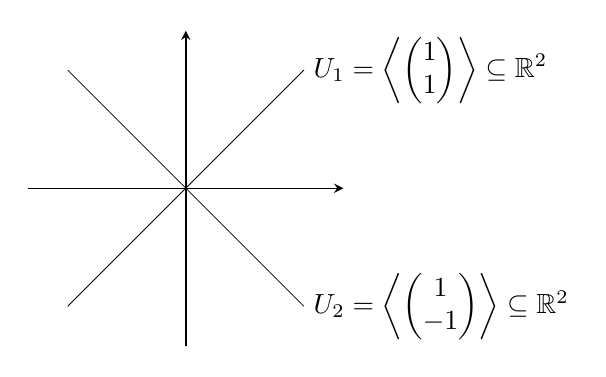
\begin{tikzpicture}
      \draw[line width=0.5pt, ->, >=stealth] (-2, 0) -- (2, 0);
      \draw[line width=0.5pt, ->, >=stealth] (0, -2) -- (0, 2);
      \draw[line width=0.3pt] (-1.5, -1.5) -- (1.5,  1.5) node[right]{$U_1=\left\langle\begin{pmatrix}1\\1\end{pmatrix}\right\rangle\subseteq\mathbb{R}^2$};
      \draw[line width=0.3pt] (-1.5,  1.5) -- (1.5, -1.5) node[right]{$U_2=\left\langle\begin{pmatrix}1\\-1\end{pmatrix}\right\rangle\subseteq\mathbb{R}^2$};
    \end{tikzpicture}
  \end{center}
  \begin{mytemize}
    \item das Beispiel zeigt zwei Geraden als Untervektorräume der Ebene $\mathbb{R}^2$
    \item die Vereinigung $U_1\cup U_2=\left\{(x,y)\in\mathbb{R}^2\mid x\in U_1\;\lor\;x\in U_2\right\}$
          besteht aus allen Vektoren, die auf beiden Geraden liegen
    \item aber mit
          \begin{equation*}
            a=
            \begin{pmatrix}
              1 \\
              1
            \end{pmatrix}
            \in U_1
            \quad\text{und}\quad
            b=
            \begin{pmatrix}
               1 \\
              -1
            \end{pmatrix}
            \in U_2
            \quad\text{gilt:}\quad
            a+b=
            \begin{pmatrix}
              2 \\
              0
            \end{pmatrix}
            \neq U_1\cup U_2
          \end{equation*}
  \end{mytemize}
  Aussage c) ist falsch:
  \begin{mytemize}
    \item jeder Untervektorraum muss den Nullvektor enthalten
    \item durch $U_1\setminus U_2$ wird also (mindestens) der Nullvektor aus $U_1$ entfernt
    \item damit kann $U_1\setminus U_2$ kein Untervektorraum mehr sein
  \end{mytemize}
\end{answer}

% ----------------------------------------------------------
\exercise{Probeklausur 30.07.2018 -- Aufgabe 7}{[10 Punkte]}
% ----------------------------------------------------------
Sei $V$ der Vektorraum aller Funktionen $\mathbb{R}\to\mathbb{R}$.
Welche der folgenden Teilmengen sind Unterräume? (Ohne Beweis)
\begin{enumerate}[a)]
  \item $M_1=\{f\in V\mid f(1)=f(-1)\}$
  \item $M_2=\{f\in V\mid f(0)\cdot f(1)=0\}$
  \item $M_3=\{f\in V\mid f(0)=1\}$
\end{enumerate}
\begin{answer}
  a) Die Menge $M_1$ bildet einen Untervektorraum von $V$:
  \begin{equation*}
    \begin{split}
      f,g\in M_1\quad&\Rightarrow\quad f(1)=f(-1)\quad\text{und}\quad g(1)=g(-1)\\[2ex]
      \big(f+g\big)(1)&=f(1)+g(1)=f(-1)+g(-1)=\big(f+g\big)(-1)\\[1ex]
      \big(k\cdot f\big)(1)&=k\cdot f(1)=k\cdot f(-1)=\big(k\cdot f\big)(-1)
    \end{split}
  \end{equation*}
  \vspace*{-\bigskipamount}%
  \begin{mytemize}
    \item $M_1$ ist also abgeschlossen bezüglich Addition und Multiplikation
  \end{mytemize}\medskip
  b) Die Menge $M_2$ bildet keinen Untervektorraum von $V$:
  \begin{alignat*}{4}
    f(x)&=x   & \quad&\Rightarrow\quad & f(0)\cdot f(1)&=0\cdot1=0 & \quad&\Rightarrow\quad f\in M_2 \\
    g(x)&=1-x & \quad&\Rightarrow\quad & g(0)\cdot g(1)&=1\cdot0=0 & \quad&\Rightarrow\quad g\in M_2
  \end{alignat*}
  \vspace*{-\bigskipamount}%
  \begin{mytemize}
    \item für die Abgeschlossenheit bezüglich der Addition müsste gelten $\big(f+g\big)(0)\cdot\big(f+g\big)(1)=0$
    \item aber: $f+g=x+1-x=1$ für alle $x\in\mathbb{R}$
  \end{mytemize}\medskip
  c) Die Menge $M_3$ bildet keinen Untervektorraum von $V$:
  \begin{equation*}
    f(x)=1 \quad\Rightarrow\quad f(0)=1 \quad\Rightarrow\quad f\in M_3
  \end{equation*}
  \vspace*{-\bigskipamount}%
  \begin{mytemize}
    \item für die Abgeschlossenheit bezüglich der Addition müsste gelten $\big(f+g\big)(0)=1$
    \item aber: $f+f=2$ für alle $x\in\mathbb{R}$
  \end{mytemize}
\end{answer}

% --------------------------------
\newsheet{Probeklausur 31.07.2018}
% --------------------------------

% ----------------------------------------------------------
\exercise{Probeklausur 31.07.2018 -- Aufgabe 1}{[10 Punkte]}
% ----------------------------------------------------------
Bestimmen Sie den Rang der folgenden Matrix.
\begin{equation*}
  \begin{pmatrix}
     1 &  4 &  5 & 0 \\
    -1 &  0 & -1 & 0 \\
     3 & -2 &  1 & 0 \\
     2 &  3 &  5 & 1
  \end{pmatrix}
\end{equation*}
\begin{answer}
  \newcommand{\matnum}[1]{\makebox[0pt][r]{{\small#1}\hspace*{1.5em}}}%
  \newcommand{\matmod}[1]{\makebox[0pt][l]{\hspace*{1.5em}\ensuremath{|{}#1}}}%
  \newcolumntype{N}{p{0pt}}%
  \newcolumntype{B}{>{\hspace*{\fill}}p{1em}}%
  \newcolumntype{R}{>{\hspace*{\fill}}p{2em}}%
  \newcolumntype{E}{p{2pt}}%
  \setlength{\arraycolsep}{0pt}%
  \begin{equation*}
    \begin{split}
      &\left(
      \begin{array}{NBRRRE}
        \matnum{I}   &  1 &  4 &  5 & 0 &                          \\
        \matnum{II}  & -1 &  0 & -1 & 0 & \matmod{+\text{I}}       \\
        \matnum{III} &  3 & -2 &  1 & 0 & \matmod{-3\cdot\text{I}} \\
        \matnum{IV}  &  2 &  3 &  5 & 1 & \matmod{-2\cdot\text{I}}
      \end{array}
      \right)\\[2ex]
      &\left(
      \begin{array}{NBRRRE}
        \matnum{I}   & 1 &   4 &   5 & 0 & \\
        \matnum{II}  & 0 &   4 &   4 & 0 & \\
        \matnum{III} & 0 & -14 & -14 & 0 & \\
        \matnum{IV}  & 0 &  -5 &  -5 & 1 &
      \end{array}
      \right)
    \end{split}
  \end{equation*}
  \begin{mytemize}
    \item An dieser Stelle erkennt man schon, dass die Zeilen II und III
          (als einzige) linear abhängig sind. Der Rang der Matrix beträgt also 3.
  \end{mytemize}
\end{answer}

% ---------------------------------------------------------
\exercise{Probeklausur 31.07.2018 -- Aufgabe 2}{[6 Punkte]}
% ---------------------------------------------------------
Bestimmen Sie mit Hilfe des Dimensionssatzes $\dim(\ker(\varphi))$ für
\begin{enumerate}[a)]
  \item $\varphi:K^6\to K^3$, mit $\varphi$ surjektiv
  \item $\varphi:K^4\to K^7$, mit $\dim(\operatorname{bild}(\varphi))=3$
  \item $\varphi:M_{2\times2}(K)\to M_{2\times2}(K)$, mit $\dim(\operatorname{bild}(\varphi))=1$
\end{enumerate}
\begin{answer}
  Abbildung a)
  \begin{mytemize}
    \item da $\varphi$ surjektiv ist, gilt: $\dim\big(\operatorname{bild}(\varphi)\big)=3$
    \item daraus folgt: $\dim\big(\ker(\varphi)\big)=\dim\big(K^6\big)-\dim\big(\operatorname{bild}(\varphi)\big)=6-3=3$
  \end{mytemize}
  Abbildung b)
  \begin{mytemize}
    \item nach Vorraussetzung gilt: $\dim\big(\operatorname{bild}(\varphi)\big)=3$
    \item daraus folgt: $\dim\big(\ker(\varphi)\big)=\dim\big(K^4\big)-\dim\big(\operatorname{bild}(\varphi)\big)=4-3=1$
  \end{mytemize}
  Abbildung c)
  \begin{mytemize}
    \item nach Vorraussetzung gilt: $\dim\big(\operatorname{bild}(\varphi)\big)=1$
    \item daraus folgt: $\dim\big(\ker(\varphi)\big)=\dim\big(M_{2\times2}(K)\big)-\dim\big(\operatorname{bild}(\varphi)\big)=4-1=3$
  \end{mytemize}
\end{answer}

% ---------------------------------------------------------
\exercise{Probeklausur 31.07.2018 -- Aufgabe 3}{[8 Punkte]}
% ---------------------------------------------------------
Bestimmen Sie mit Hilfe der Determinanten, für welche $k\in\mathbb{R}$
die Matrix
\begin{equation*}
  \begin{pmatrix}
    k & 1 & 0 & -k \\
    0 & 1 & 0 &  0 \\
    0 & 1 & 1 &  0 \\
    k & 0 & 0 &  1
  \end{pmatrix}
  \in M_{4\times4}(\mathbb{R})
\end{equation*}
invertierbar ist.
\begin{answer}
  \begin{mytemize}
    \item Die Entwicklung der Determinanten nach einer Zeile erfolge gemäß der Gleichung
          \begin{equation*}
            \det(A)=\sum_{j=1}^n(-1)^{i+j}a_{ij}\det(A_{ij})\;,
          \end{equation*}
          wobei $A_{ij}$ die Matrix bezeichnet, die aus $A$ entsteht, wenn man die
          $i$-te Zeile und die $j$-te Spalte streicht.
    \item Die Entwicklung nach der 2. Zeile ergibt hier also:
          \begin{equation*}
            \begin{split}
              \det(A)&=\sum_{j=1}^4(-1)^{2+j}a_{2j}\det(A_{2j})
                      =(-1)^{2+2}a_{22}\det(A_{22})\\[1ex]
              &=\det
              \begin{pmatrix}
                k & 0 & -k \\
                0 & 1 &  0 \\
                k & 0 &  1
              \end{pmatrix}
              =k+k^2=k(1+k)
            \end{split}
          \end{equation*}
    \item Eine Matrix ist genau dann invertierbar, falls die Determinante nicht Null ist:
          \begin{equation*}
              0\neq k(1+k)\quad\Rightarrow\quad k\in\mathbb{R}\setminus\{0,-1\}
          \end{equation*}
  \end{mytemize}
\end{answer}

% ---------------------------------------------------------
\exercise{Probeklausur 31.07.2018 -- Aufgabe 4}{[8 Punkte]}
% ---------------------------------------------------------
Finden Sie das Inverse zu folgender Matrix:
\begin{equation*}
  \begin{pmatrix}
    1 & 1 & 0 \\
    1 & 1 & 1 \\
    0 & 1 & 1
  \end{pmatrix}
\end{equation*}
\begin{answer}
  \newcommand{\matnum}[1]{\makebox[0pt][r]{{\small#1}\hspace*{1.5em}}}%
  \newcommand{\matmod}[1]{\makebox[0pt][l]{\hspace*{1.5em}\ensuremath{|{}#1}}}%
  \newcolumntype{N}{p{0pt}}%
  \newcolumntype{B}{>{\hspace*{\fill}}p{0.6em}}%
  \newcolumntype{R}{>{\hspace*{\fill}}p{1.5em}}%
  \newcolumntype{E}{p{2pt}}%
  \newcolumntype{S}{p{10pt}}%
  \setlength{\arraycolsep}{0pt}%
  \begin{equation*}
    \begin{split}
      &\left(
      \begin{array}{NBRRS|RRRE}
        \matnum{I}   & 1 & 1 & 0 && 1 & 0 & 0 &                    \\
        \matnum{II}  & 1 & 1 & 1 && 0 & 1 & 0 & \matmod{-\text{I}} \\
        \matnum{III} & 0 & 1 & 1 && 0 & 0 & 1 &
      \end{array}
      \right)\\[2ex]
      &\left(
      \begin{array}{NBRRS|RRRE}
        \matnum{I}   & 1 & 1 & 0 &&  1 & 0 & 0 &                               \\
        \matnum{II}  & 0 & 0 & 1 && -1 & 1 & 0 & \matmod{\leftarrow\text{III}} \\
        \matnum{III} & 0 & 1 & 1 &&  0 & 0 & 1 & \matmod{\leftarrow\text{II}}
      \end{array}
      \right)\\[2ex]
      &\left(
      \begin{array}{NBRRS|RRRE}
        \matnum{I}   & 1 & 1 & 0 &&  1 & 0 & 0 &                      \\
        \matnum{II}  & 0 & 1 & 1 &&  0 & 0 & 1 & \matmod{-\text{III}} \\
        \matnum{III} & 0 & 0 & 1 && -1 & 1 & 0 &
      \end{array}
      \right)\\[2ex]
      &\left(
      \begin{array}{NBRRS|RRRE}
        \matnum{I}   & 1 & 1 & 0 &&  1 &  0 & 0 & \matmod{-\text{II}} \\
        \matnum{II}  & 0 & 1 & 0 &&  1 & -1 & 1 &                     \\
        \matnum{III} & 0 & 0 & 1 && -1 &  1 & 0 &
      \end{array}
      \right)\\[2ex]
      &\left(
      \begin{array}{NBRRS|RRRE}
        \matnum{I}   & 1 & 0 & 0 &&  0 &  1 & -1 & \\
        \matnum{II}  & 0 & 1 & 0 &&  1 & -1 &  1 & \\
        \matnum{III} & 0 & 0 & 1 && -1 &  1 &  0 &
      \end{array}
      \right)\\[2ex]
    \end{split}
  \end{equation*}
\end{answer}

% ---------------------------------------------------------
\exercise{Probeklausur 31.07.2018 -- Aufgabe 5}{[6 Punkte]}
% ---------------------------------------------------------
Seien $A$, $B$ und $S$ $n\times n$ Matrizen, $S$ invertierbar und $A=S^{-1}BS$.
Begründen Sie ausführlich, warum $\det(A)=\det(B)$ gilt.
\begin{answer}
  \begin{equation*}
    \begin{split}
      \det(A)&=\det(S^{-1}BS)\\
      &=\det(S^{-1})\cdot\det(B)\cdot\det(S)\qquad\text{dies sind drei reelle Zahlen}\\
      &=\det(S)^{-1}\cdot\det(S)\cdot\det(B)\\[1ex]
      &=\frac{\det(S)}{\det(S)}\cdot\det(B)=\det(B)
    \end{split}
  \end{equation*}
\end{answer}

% ---------------------------------------------------------
\exercise{Probeklausur 31.07.2018 -- Aufgabe 6}{[9 Punkte]}
% ---------------------------------------------------------
Zeigen Sie:
\begin{enumerate}[a)]
  \item Ist $A\in M_{n\times n}(K)$ eine invertierbare Matrix und $k\in K$
        mit $k\neq0$, so ist auch $kA$ invertierbar.
  \item Ist $A^2=0$, so sind auch $I_n-A$ und $I_n+A$ invertierbar.
\end{enumerate}
Geben Sie außerdem ein Beispiel an, das zeigt, dass die folgende
Aussage falsch ist:
\begin{enumerate}[a)]
  \setcounter{enumi}{2}
  \item Sind $A,B\in M_{n\times n}(K)$ invertierbar, so ist auch $A+B$
        invertierbar.
\end{enumerate}
\begin{answer}
  Begründung zu a)
  \begin{equation*}
    \det(k\cdot A)=k^n\cdot\det(A)
  \end{equation*}
  \begin{mytemize}
    \item weil $A$ nach Vorraussetzung invertierbar ist, gilt $\det(A)\neq0$
    \item nach Vorraussetzung ist $k\neq0$, also auch $k^n\neq0$
    \item also ist auch $\det(k\cdot A)\neq0$ und $k\cdot A$ damit invertierbar
  \end{mytemize}
  \par
  Begründung zu b)
  \begin{equation*}
    \begin{split}
      A^2=0&\Rightarrow\det\big(I_n-A^2\big)\neq0\\
           &\Rightarrow\det\big(I_n-A+A-A^2\big)\neq0\\
           &\Rightarrow\det\big((I_n-A)\cdot I_n+(I_n-A)\cdot A\big)\neq0\\
           &\Rightarrow\det\big((I_n-A)\cdot(I_n+A)\big)\neq0\\
           &\Rightarrow\det(I_n-A)\cdot\det(I_n+A)\neq0\\
           &\Rightarrow(I_n\pm A)\text{ sind invertierbar}
    \end{split}
  \end{equation*}
  \begin{mytemize}
    \item das Ausmultiplizieren von $(I_n-A)\cdot(I_n+A)$ hat zur Lösung geführt\ldots
  \end{mytemize}
  \par
  Gegenbeispiel zu c)
  \begin{equation*}
    A=
    \begin{pmatrix}
      1 & 0 & 0 \\
      0 & 1 & 0 \\
      0 & 0 & 1
    \end{pmatrix}
    \quad
    \det(A)=1
    \qquad
    \qquad
    B=
    \begin{pmatrix}
      1 &  0 & 0 \\
      0 & -1 & 0 \\
      0 &  0 & 1
    \end{pmatrix}
    \quad
    \det(B)=-1
  \end{equation*}
  \begin{mytemize}
    \item beide Matritzen sind invertierbar, da beide Determinanten ungleich Null sind
  \end{mytemize}
  \begin{equation*}
    \det(A+B)=\det
    \begin{pmatrix}
      2 & 0 & 0 \\
      0 & 0 & 0 \\
      0 & 0 & 2
    \end{pmatrix}
    =0
  \end{equation*}
  \begin{mytemize}
    \item also ist die Matrix $C=A+B$ nicht invertierbar
  \end{mytemize}
\end{answer}

% ----------------------------------------------------------
\exercise{Probeklausur 31.07.2018 -- Aufgabe 7}{[12 Punkte]}
% ----------------------------------------------------------
Sei $\varphi:V\to W$ eine lineare Abbildung zwischen Vektorräumen.
Beweisen oder widerlegen Sie:
\begin{enumerate}[a)]
  \item Sind $v_1,\ldots,v_n$ Eigenvektoren mit dem gleichen Eigenwert $k$,
        so ist jeder nicht-triviale Vektor aus $\langle v_1,\ldots,v_n\rangle$
        Eigenvektor zum Eigenwert $k$.
  \item Ist $v$ ein Eigenvektor mit Eigenwert $k$ und $w$ ein Eigenvektor
        mit Eigenwert $\ell$, so ist $v+w$ Eigenvektor mit Eigenwert $k+\ell$.
  \item Ist $v$ ein Eigenvektor von $\varphi$ und gleichzeitig auch Eigenvektor
        von $\psi:W\to U$, so ist $v$ auch Eigenvektor von $\psi\circ\varphi$.
  \item Ist $k$ ein Eigenwert von $\varphi$ und gleichzeitig auch Eigenwert von
        $\psi:W\to U$, so ist $k$ auch Eigenwert von $\psi\circ\varphi$.
\end{enumerate}
\begin{answer}
  Aussage a) ist wahr:
  \begin{equation*}
    \begin{split}
      \text{Mit }\nu&=a_1v_1+a_2v_2+\cdots+a_nv_n\in\langle v_1,\ldots,v_n\rangle\text{ gilt:}\\[1ex]
      \varphi(\nu)&=\varphi(a_1v_1+a_2v_2+\cdots+a_nv_n)\\
                  &=a_1\varphi(v_1)+a_2\varphi(v_2)+\cdots+a_n\varphi(v_n)\\
                  &=a_1k v_1+a_2k v_2+\cdots+a_nk v_n\\
                  &=k\cdot(a_1v_1+a_2v_2+\cdots+a_nv_n)\\
                  &=k\cdot\nu
    \end{split}
  \end{equation*}
  Aussage b) ist falsch:
  \begin{equation*}
    A=
    \begin{pmatrix}
      k &    0 \\
      0 & \ell
    \end{pmatrix}
    \qquad
    \det(A-\lambda I)=(k-\lambda)(\ell-\lambda)=0
    \quad\Rightarrow\quad
    \lambda_1=k\;,\;\lambda_2=\ell
  \end{equation*}
  \begin{mytemize}
    \item aber diese Matrix besitzt gar keinen Eigenwert $k+\ell$
  \end{mytemize}
  Aussage c) ist wahr:
  \begin{equation*}
    \begin{split}
      \varphi(v)&=\lambda\cdot v\\
      \psi(v)&=\mu\cdot v\\
      \psi(\varphi(v))&=\psi(\lambda v)=\lambda\cdot\psi(v)=\lambda\mu\cdot v
    \end{split}
  \end{equation*}
  Aussage d) ist falsch:
  \begin{equation*}
    \varphi(x)=
    \begin{pmatrix}
      k & 0 \\
      0 & 1
    \end{pmatrix}
    \cdot x
    \qquad
    \psi(x)=
    \begin{pmatrix}
      k & 0 \\
      0 & 2
    \end{pmatrix}
    \cdot x
    \qquad
    \big(\psi\circ\varphi\big)(x)=
    \psi(\varphi(x))=
    \begin{pmatrix}
      k^2 & 0 \\
      0   & 2
    \end{pmatrix}
    \cdot x
  \end{equation*}
  \begin{mytemize}
    \item $k$ ist also nicht automatisch auch ein Eigenwert von $\psi\circ\varphi$
  \end{mytemize}
\end{answer}

% ----------------------------------------------------------
\exercise{Probeklausur 31.07.2018 -- Aufgabe 8}{[16 Punkte]}
% ----------------------------------------------------------
Finden Sie alle Eigenwerte der folgenden Matrix $A\in M_{3\times3}(\mathbb{R})$
und bestimmen Sie zu jedem Eigenwert einen Eigenvektor.
\begin{equation*}
  A=
  \begin{pmatrix}
     1 & -1 &  0 \\
    -1 &  2 & -1 \\
     0 & -1 &  1
  \end{pmatrix}
\end{equation*}
\begin{answer}
  Eigenwerte:
  \begin{equation*}
    \begin{split}
      \det(A-\lambda I)
      &=\det
      \begin{pmatrix}
        1-\lambda &        -1 &         0 \\
               -1 & 2-\lambda &        -1 \\
                0 &        -1 & 1-\lambda
      \end{pmatrix}
      =0\\[2ex]
      &=(1-\lambda)(2-\lambda)(1-\lambda)-(-1)(-1)(1-\lambda)-(1-\lambda)(-1)(-1)\\
      &=(1-\lambda)(2-\lambda)(1-\lambda)-(1-\lambda)-(1-\lambda)\\
      &=(1-\lambda)\big[(2-\lambda)(1-\lambda)-2\big]\\
      &=(1-\lambda)\big[2-2\lambda-\lambda+\lambda^2-2\big]\\
      &=(1-\lambda)\big[\lambda^2-3\lambda\big]\\
      &=(1-\lambda)\cdot\lambda\cdot(\lambda-3)\\[1ex]
      \Rightarrow\quad\lambda_1&=0\;,\;\lambda_2=1\;,\;\lambda_3=3
    \end{split}
  \end{equation*}
  Eigenvektor zu $\lambda_1=0$:
  \begin{equation*}
    \begin{pmatrix}
       1 & -1 &  0 \\
      -1 &  2 & -1 \\
       0 & -1 &  1
    \end{pmatrix}
    \cdot
    \begin{pmatrix}
      x \\
      y \\
      z
    \end{pmatrix}
    =
    \begin{pmatrix}
      0 \\
      0 \\
      0
    \end{pmatrix}
  \end{equation*}
  \begin{mytemize}
    \item aus Zeile I folgt: $x=y$
    \item aus Zeile III folgt: $y=z$
    \item also gilt insgesamt:
  \end{mytemize}
  \begin{equation*}
    v_1=t\cdot
    \begin{pmatrix}
      1 \\
      1 \\
      1
    \end{pmatrix}
    \quad\text{mit}\quad
    t\in\mathbb{R}\setminus\{0\}
  \end{equation*}
  Eigenvektor zu $\lambda_2=1$:
  \begin{equation*}
    \begin{pmatrix}
       0 & -1 &  0 \\
      -1 &  1 & -1 \\
       0 & -1 &  0
    \end{pmatrix}
    \cdot
    \begin{pmatrix}
      x \\
      y \\
      z
    \end{pmatrix}
    =
    \begin{pmatrix}
      0 \\
      0 \\
      0
    \end{pmatrix}
  \end{equation*}
  \begin{mytemize}
    \item aus Zeile I und III folgt: $y=0$
    \item damit folgt aus Zeile II: $x=-z$
    \item also gilt insgesamt:
  \end{mytemize}
  \begin{equation*}
    v_2=t\cdot
    \begin{pmatrix}
       1 \\
       0 \\
      -1
    \end{pmatrix}
    \quad\text{mit}\quad
    t\in\mathbb{R}\setminus\{0\}
  \end{equation*}
  Eigenvektor zu $\lambda_3=3$:
  \begin{equation*}
    \begin{pmatrix}
      -2 & -1 &  0 \\
      -1 & -1 & -1 \\
       0 & -1 & -2
    \end{pmatrix}
    \cdot
    \begin{pmatrix}
      x \\
      y \\
      z
    \end{pmatrix}
    =
    \begin{pmatrix}
      0 \\
      0 \\
      0
    \end{pmatrix}
  \end{equation*}
  \begin{mytemize}
    \item aus Zeile I folgt: $y=-2x$
    \item aus Zeile III folgt: $y=-2z$
    \item daraus folgt: $x=z$
    \item also gilt insgesamt:
  \end{mytemize}
  \begin{equation*}
    v_3=t\cdot
    \begin{pmatrix}
       1 \\
      -2 \\
       1
    \end{pmatrix}
    \quad\text{mit}\quad
    t\in\mathbb{R}\setminus\{0\}
  \end{equation*}
\end{answer}

% ---------------------------
\newsheet{Klausur 11.09.2014}
% ---------------------------

% ----------------------------------------------------
\exercise{Klausur 11.09.2014 -- Aufgabe 1}{[7 Punkte]}
% ----------------------------------------------------
Wir betrachten das lineare Gleichungssystem über den reellen Zahlen:
\begin{equation*}
  \newcommand{\+}{&{}+{}&}%
  \renewcommand{\-}{&{}-{}&}%
  \renewcommand{\=}{&{}={}&}%
  \renewcommand{\.}{&{}~{}&}%
  \renewcommand{\|}{\text{\;\;}&}%
  \setlength{\arraycolsep}{0pt}%
  \begin{array}{|crcrcrcrcr}
  \| 3x_1 \+ 4x_2 \+ 2x_3 \+  2x_4 \=  2 \\
  \| 2x_1 \+ 2x_2 \+ 4x_3 \+  3x_4 \=  4 \\
  \| 3x_1 \+ 3x_2 \+ 3x_3 \+ a x_4 \=  1 \\
  \| 3x_1 \+ 6x_2 \+ 6x_3 \+  7x_4 \= 10   
  \end{array}
\end{equation*}
\begin{enumerate}[a)]
  \item Für welche Werte der Parameters $a\in\mathbb{R}$ ist das Gleichungssystem lösbar?
  \item Berechnen Sie die Lösung für den Wert $a=1$.
\end{enumerate}
\begin{answer}
  Teilaufgabe a)
  \begin{mytemize}
    \item Entwicklung der Determinanten nach der Zeile, in der der Parameter $a$ vorkommt:
  \end{mytemize}
    \begin{equation*}
      \begin{split}
        A&=
        \begin{pmatrix}
          3 & 4 & 2 & 2 \\
          2 & 2 & 4 & 3 \\
          3 & 3 & 3 & a \\
          3 & 6 & 6 & 7
        \end{pmatrix}\\
        \det(A)&=(-1)^{3+1}\cdot3\cdot\det
        \begin{pmatrix}
          4 & 2 & 2 \\
          2 & 4 & 3 \\
          6 & 6 & 7
        \end{pmatrix}
        +(-1)^{3+2}\cdot3\cdot\det
        \begin{pmatrix}
          3 & 2 & 2 \\
          2 & 4 & 3 \\
          3 & 6 & 7
        \end{pmatrix}\\
        &+(-1)^{3+3}\cdot3\cdot\det
        \begin{pmatrix}
          3 & 4 & 2 \\
          2 & 2 & 3 \\
          3 & 6 & 7
        \end{pmatrix}
        +(-1)^{3+3}\cdot a\cdot\det
        \begin{pmatrix}
          3 & 4 & 2 \\
          2 & 2 & 4 \\
          3 & 6 & 6
        \end{pmatrix}\\
        &=3\cdot(4\cdot4\cdot7+2\cdot3\cdot6+2\cdot2\cdot6-6\cdot4\cdot2-6\cdot3\cdot4-7\cdot2\cdot2)\\
        &-3\cdot(3\cdot4\cdot7+2\cdot3\cdot3+2\cdot2\cdot6-3\cdot4\cdot2-6\cdot3\cdot3-7\cdot2\cdot2)\\
        &+3\cdot(3\cdot2\cdot7+4\cdot3\cdot3+2\cdot2\cdot6-3\cdot2\cdot2-6\cdot3\cdot3-7\cdot2\cdot4)\\
        &-a\cdot(3\cdot2\cdot6+4\cdot4\cdot3+2\cdot2\cdot6-3\cdot2\cdot2-6\cdot4\cdot3-6\cdot2\cdot4)\\
        &=24a-48\neq0\quad\Rightarrow\quad a\neq2
      \end{split}
    \end{equation*}
    \begin{mytemize}
      \item das Gleichungssystem ist also für alle $a\in\mathbb{R}\setminus\{2\}$ lösbar
    \end{mytemize}
    Teilaufgabe b)
    \begin{equation*}
      \newcommand{\+}{&{}+{}&}%
      \renewcommand{\-}{&{}-{}&}%
      \renewcommand{\=}{&{}={}&}%
      \renewcommand{\.}{&{}~{}&}%
      \renewcommand{\|}{\text{\;\;}&}%
      \setlength{\arraycolsep}{0pt}%
      \begin{array}{|crcrcrcrcr}
      \| 3x_1 \+ 4x_2 \+ 2x_3 \+ 2x_4 \=  2 \\
      \| 2x_1 \+ 2x_2 \+ 4x_3 \+ 3x_4 \=  4 \\
      \| 3x_1 \+ 3x_2 \+ 3x_3 \+  x_4 \=  1 \\
      \| 3x_1 \+ 6x_2 \+ 6x_3 \+ 7x_4 \= 10   
      \end{array}
      \qquad\Rightarrow\qquad
      x=
      \frac{1}{2}\cdot
      \begin{pmatrix}
        -2 \\
         1 \\
         1 \\
         2
      \end{pmatrix}
    \end{equation*}
\end{answer}

% ----------------------------------------------------
\exercise{Klausur 11.09.2014 -- Aufgabe 2}{[7 Punkte]}
% ----------------------------------------------------
Im Vektorraum $\mathbb{R}^4$ seien folgende Vektoren gegeben
\begin{equation*}
  v_1=
  \begin{pmatrix}
     1 \\
     2 \\
    -1 \\
     2
  \end{pmatrix}
  \;,\quad
  v_2=
  \begin{pmatrix}
    2 \\
    1 \\
    2 \\
    1
  \end{pmatrix}
  \;,\quad
  v_3=
  \begin{pmatrix}
    -1 \\
     2 \\
     1 \\
     2
  \end{pmatrix}
  \;,\quad
  w_1=
  \begin{pmatrix}
    2 \\
    1 \\
    1 \\
    2
  \end{pmatrix}
  \quad\text{und}\quad
  w_2=
  \begin{pmatrix}
    1 \\
    1 \\
    2 \\
    2
  \end{pmatrix}
  \;,
\end{equation*}
die die Unterräume $U_1=\langle v_1,v_2,v_3\rangle$ und $U_2=\langle w_1,w_2\rangle$ erzeugen.
\begin{enumerate}[a)]
  \item Bestimmen Sie eine lineare Gleichung für $U_1$ (d.\,h. $U_1$ soll die Lösungsmenge sein).
  \item Bestimmen Sie eine Basis des Durchschnitts $U_1\cap U_2$ mit einer Methode Ihrer Wahl.
\end{enumerate}
\begin{answer}
  Teilaufbage b)
  \begin{mytemize}
    \item alle Vektoren, die sich im Schnitt der beiden Unterräume
          befinden, müssen sich sowohl als Linearkombination von $\langle
          v_1,v_2,v_3\rangle$, als auch von $\langle w_1,w_2\rangle$ darstellen
          lassen, also:
          \begin{equation*}
            a\cdot v_1+b\cdot v_2+c\cdot v_3=d\cdot w_1+e\cdot w_2
            \quad\Rightarrow\quad
            a\cdot v_1+b\cdot v_2+c\cdot v_3-d\cdot w_1-e\cdot w_2=0
          \end{equation*}
    \item dieses Gleichungssystem lässt sich mit 'Gauß' lösen:
          \begin{equation*}
            \newcommand{\+}{&{}+{}&}%
            \renewcommand{\-}{&{}-{}&}%
            \renewcommand{\=}{&{}={}&}%
            \renewcommand{\.}{&{}~{}&}%
            \renewcommand{\|}{\text{\;\;}&}%
            \setlength{\arraycolsep}{0pt}%
            \begin{array}{|crcrcrcrcrcr}
            \|  a \+ 2b \-  c \- 2d \-  e \= 0 \\
            \| 2a \+  b \+ 2c \-  d \-  e \= 0 \\
            \| -a \+ 2b \+  c \-  d \- 2e \= 0 \\
            \| 2a \+  b \+ 2c \- 2d \- 2e \= 0   
            \end{array}
            \qquad\Rightarrow\qquad
            x=t\cdot
            \begin{pmatrix}
               1 \\
               0 \\
              -1 \\
               2 \\
              -2
            \end{pmatrix}
            \text{ mit }t\in\mathbb{R}
          \end{equation*}
    \item der Schnitt hat also folgende eindimensionale Basis:
          \begin{equation*}
            \stretchleftright
            {\hstretch{2}{\langle}}%
            {%
              \begin{pmatrix}
                 1 \\
                 0 \\
                -1 \\
                 2 \\
                -2
              \end{pmatrix}
            }%
            {\hstretch{2}{\rangle}}%
          \end{equation*}
  \end{mytemize}
\end{answer}

% ----------------------------------------------------
\exercise{Klausur 11.09.2014 -- Aufgabe 3}{[7 Punkte]}
% ----------------------------------------------------
\begin{enumerate}[a)]
  \item Berechnen Sie die Inverse der folgenden reellen Matrix:
        \begin{equation*}
          A=
          \begin{pmatrix}
            0 & 1 & 0 & 1 \\
            1 & 0 & 1 & 1 \\
            0 & 1 & 1 & 0 \\
            1 & 1 & 0 & 0
          \end{pmatrix}
        \end{equation*}
  \item Begründen Sie, dass die reelle Matrix
        \begin{equation*}
          B=
          \begin{pmatrix}
            0 & 1 & 0 & 1 \\
            1 & 0 & 1 & 0 \\
            0 & 1 & 0 & 1 \\
            1 & 0 & 1 & 0
          \end{pmatrix}
        \end{equation*}
        nicht invertierbar ist.
\end{enumerate}

% ----------------------------------------------------
\exercise{Klausur 11.09.2014 -- Aufgabe 4}{[7 Punkte]}
% ----------------------------------------------------
\begin{enumerate}[a)]
  \item Berechnen Sie (auf günstige Weise) die Determinante der reellen Matrix
        \begin{equation*}
          A=
          \begin{pmatrix}
             2 &  3 &  5 &  2 \\
             3 &  2 &  3 & -2 \\
             2 &  a &  2 &  2 \\
            -2 & -3 & -2 & -3
          \end{pmatrix}
        \end{equation*}
        mit dem Parameter $a\in\mathbb{R}$.
  \item Für welche $a\in\mathbb{R}$ ist die Matrix nicht invertierbar?
\end{enumerate}

% ----------------------------------------------------
\exercise{Klausur 11.09.2014 -- Aufgabe 5}{[7 Punkte]}
% ----------------------------------------------------
Im Vektorraum $\mathbb{R}^5$ mit dem Standard-Skalarprodukt betrachten wir die Vektoren
\begin{equation*}
  v_1=
  \begin{pmatrix}
     2 \\
     1 \\
    -3 \\
    -1 \\
    -1
  \end{pmatrix}
  \qquad
  v_2=
  \begin{pmatrix}
    -4 \\
     2 \\
     2 \\
     2 \\
     2
  \end{pmatrix}
  \qquad
  v_3=
  \begin{pmatrix}
    0 \\
    5 \\
    5 \\
    3 \\
    3
  \end{pmatrix}
\end{equation*}
\begin{enumerate}[a)]
  \item Berechnen Sie eine Orthonormalbasis des Unterraums $U=\langle v_1,v_2,v_3\rangle$,
        inden Sie die gegebenen Vektoren orthonormalisieren.
  \item Geben Sie die orthogonale Projektion $P:\mathbb{R}^5\to\mathbb{R}^5$ auf den
        Unterraum $U$ (ohne nähere Ausrechnung) an und berechnen sie den Wert $P(1,0,0,0,0)$.
\end{enumerate}

% ----------------------------------------------------
\exercise{Klausur 11.09.2014 -- Aufgabe 6}{[5 Punkte]}
% ----------------------------------------------------
Sei $V$ ein Vektorraum mit der Dimension $n\in\mathbb{N}$ und $f:V\to V$
eine lineare Abbildung. Mit $f^i$ bezeichnen wir die Verkettung
$f\circ\cdots\circ f$ von $i$ Faktoren $f$ (und mit $f^0$ die identische Abbildung).
Zeigen Sie:
\begin{enumerate}[a)]
  \item Für $i\geq1$ gilt $\operatorname{bild}(f^{i+1})\subseteq\operatorname{bild}(f^i)$
  \item Wenn $\operatorname{bild}(f^{i+1})=\operatorname{bild}(f^i)$ für ein $i\geq0$
        gilt, dann gilt auch $\operatorname{bild}(f^j)=\operatorname{bild}(f^i)$
        für alle $j\geq i$.
  \item Es gibt ein $i\leq n$ mit $\operatorname{bild}(f^{i+1})=\operatorname{bild}(f^i)$.\par
        {\itshape Tipp: Was könnte man andernfalls über die Dimension der Bilder sagen?}
\end{enumerate}

% ---------------------------
\newsheet{Klausur 10.09.2015}
% ---------------------------

% ----------------------------------------------------
\exercise{Klausur 10.09.2015 -- Aufgabe 1}{[7 Punkte]}
% ----------------------------------------------------
Wir betrachten das lineare Gleichungssystem über den reellen Zahlen:
\begin{equation*}
  \newcommand{\+}{&{}+{}&}%
  \renewcommand{\-}{&{}-{}&}%
  \renewcommand{\=}{&{}={}&}%
  \renewcommand{\.}{&{}~{}&}%
  \renewcommand{\|}{\text{\;\;}&}%
  \setlength{\arraycolsep}{0pt}%
  \begin{array}{|crcrcrcrcr}
  \| 4x_1 \+ 5x_2 \+ 6x_3 \+  4x_4 \= 1 \\
  \|  x_1 \+ 2x_2 \+ 7x_3 \+  4x_4 \= 2 \\
  \| 3x_1 \+ 4x_2 \+ 3x_3 \+   x_4 \= 1 \\
  \| 4x_1 \+ 5x_2 \+ 5x_3 \+ a x_4 \= 1   
  \end{array}
\end{equation*}
\begin{enumerate}[a)]
  \item Für welche Werte des Parameters $a\in\mathbb{R}$ ist das Gleichungssystem lösbar?
  \item Berechnen Sie die Lösung für den Wert $a=3$.
\end{enumerate}
\begin{answer}
  Teilaufgabe a)
  \begin{mytemize}
    \item da der Parameter $a$ ganz rechts unten in der Matrix steht,
          muss man die Determinante nicht mit \glqq Laplace\grqq{}
          entwickeln, sondern kann direkt mit \glqq Gauss\grqq{} die
          Zeilenstufenform herstellen, die ohnehin in Teilaufgabe b)
          benötigt wird:
          \begin{equation*}
            (A\mid b)=
            \left(
            \begin{array}{rrrr|r}
              1 &  2 &   7 &      4 &  2 \\
              0 & -3 & -22 &    -12 & -7 \\
              0 &  0 & -10 &     -9 & -1 \\
              0 &  0 &   0 & 10a-31 &  1
            \end{array}
            \right)
          \end{equation*}
    \item unter Berücksichtigung der elementaren Zeilenumformungen gilt
          für die Determinante:
          \begin{equation*}
            \det(A)=-\frac{1}{30}\cdot1\cdot(-3)\cdot(-10)\cdot(10a-31)=31-10a
          \end{equation*}
    \item das Gleichungssystem ist also für alle
          $a\in\mathbb{R}\setminus\left\{\frac{31}{10}\right\}$ lösbar
  \end{mytemize}
  Teilaufgabe b)
  \begin{equation*}
    x=
    \begin{pmatrix}
       1 \\
      -1 \\
       1 \\
      -1
    \end{pmatrix}
  \end{equation*}
\end{answer}

% ----------------------------------------------------
\exercise{Klausur 10.09.2015 -- Aufgabe 2}{[7 Punkte]}
% ----------------------------------------------------
Im Vektorraum $\mathbb{R}^4$ seien die folgenden Untervektorräume gegeben:
\begin{itemize}
  \item $U_1$ ist die Lösungsmenge einer linearen Gleichung
        \begin{equation*}
          U_1=\left\{x=(x_1,x_2,x_3,x_4)^\text{t}\in\mathbb{R}^4\mid2x_1+x_2-2x_3+x_4=0\right\}
        \end{equation*}
  \item $U_2$ wird von folgenden Vektoren erzeugt
        \begin{equation*}
          w_1=
          \begin{pmatrix}
            2 \\
            2 \\
            2 \\
            1
          \end{pmatrix}
          \qquad
          w_2=
          \begin{pmatrix}
            1 \\
            3 \\
            2 \\
            2
          \end{pmatrix}
        \end{equation*}
\end{itemize}
\begin{enumerate}[a)]
  \item Bestimmen Sie eine Basis für $U_1$.
  \item Bestimmen Sie eine Basis des Durchschnitts $U_1\cap U_2$ mit
        einer Methode Ihrer Wahl.
  \item Begründen Sie (z.\,B. mit der Dimensionsformel), dass die
        Summe $U_1+U_2$ der gesamte Vektorraum $\mathbb{R}^4$ ist
\end{enumerate}
\begin{answer}
  Teilaufgabe a)
  \begin{mytemize}
    \item Auflösen der Gleichung nach einer der Unbekannten ergibt zum Beispiel:
          \begin{equation*}
            x_4=-2x_1-x_2+2x_3
          \end{equation*}
    \item also haben alle Vektoren in $U_1$ die Form:
          \begin{equation*}
            x=
            \begin{pmatrix}
                         x_1 \\
                         x_2 \\
                         x_3 \\
              -2x_1-x_2+2x_3
            \end{pmatrix}
          \end{equation*}
    \item eine mögliche Basis wäre also:
          \begin{equation*}
            \left\{
            \begin{pmatrix}
               1 \\
               0 \\
               0 \\
              -2
            \end{pmatrix}
            ,
            \begin{pmatrix}
               0 \\
               1 \\
               0 \\
              -1
            \end{pmatrix}
            ,
            \begin{pmatrix}
              0 \\
              0 \\
              1 \\
              2
            \end{pmatrix}
            \right\}
          \end{equation*}
  \end{mytemize}
  Teilaufgabe b)
  \begin{mytemize}
    \item alle Vektoren im Schnitt werden von beiden Basen erzeugt, also:
  \end{mytemize}
  Teilaufgabe c)
\end{answer}

% ----------------------------------------------------
\exercise{Klausur 10.09.2015 -- Aufgabe 3}{[7 Punkte]}
% ----------------------------------------------------
\begin{enumerate}[a)]
  \item Berechnen Sie die Inverse der folgenden reellen Matrix:
        \begin{equation*}
          A=
          \begin{pmatrix}
            0 & 1 & 0 & 1 \\
            1 & 1 & 1 & 0 \\
            0 & 1 & 1 & 1 \\
            1 & 0 & 1 & 0
          \end{pmatrix}
        \end{equation*}
  \item Bestimmen Sie den Rang der folgenden reellen Matrix:
        \begin{equation*}
          B=
          \begin{pmatrix}
            1 & 1 & 1 & 0 \\
            1 & 1 & 0 & 1 \\
            1 & 0 & 1 & 1 \\
            0 & 1 & 1 & 1
          \end{pmatrix}
        \end{equation*}
\end{enumerate}

% ----------------------------------------------------
\exercise{Klausur 10.09.2015 -- Aufgabe 4}{[7 Punkte]}
% ----------------------------------------------------
\begin{enumerate}[a)]
  \item Berechnen Sie (auf günstige Weise) die Determinante der folgenden
        reellen Matrix mit dem Parameter $a\in\mathbb{R}$:
        \begin{equation*}
          A=
          \begin{pmatrix}
            2 & 3 & -2 &  3 \\
            3 & 2 &  2 & -2 \\
            3 & a &  3 &  3 \\
            2 & 2 &  3 & -2
          \end{pmatrix}
        \end{equation*}
  \item Für welche $a\in\mathbb{R}$ besitzt die Matrix \emph{keine} inverse Matrix?
\end{enumerate}

% ----------------------------------------------------
\exercise{Klausur 10.09.2015 -- Aufgabe 5}{[7 Punkte]}
% ----------------------------------------------------
Wir betrachten im Folgenden Permutationen aus der Gruppe $S_{10}$
(aller Permutationen der Zahlen $1,\ldots,10$):
\begin{equation*}
  \begin{split}
    \sigma_1&=
    \begin{pmatrix}
      1 & 2 & 3 & 4 & 5 & 6 &  7 & 8 & 9 & 10 \\
      3 & 4 & 5 & 6 & 1 & 2 & 10 & 9 & 8 &  7
    \end{pmatrix}
    \\[1ex]
    \sigma_2&=\langle1,2,3,4,5\rangle\langle3,4,5,6,7\rangle\langle5,6,7,8,9,10\rangle
  \end{split}
\end{equation*}
Die erste Angabe ist eine Wertetabelle, die zweite eine \emph{nicht
kanonische} Darstellung durch Zyklen. Man beachte, dass die Verkettung
von rechts nach links ausgewertet wird.
\begin{enumerate}[a)]
  \item Bestimmen Sie für beide Permutationen:
        \begin{itemize}
          \item Die kanonische Zyklendarstellung.
          \item Eine Darstellung durch Transpositionen.
          \item Das Signum.
        \end{itemize}
  \item Berechnen Sie die Ordnung von $\sigma_1$, d.\,h. die kleinste
        Zahl $m\geq1$ mit $\sigma_1^m=\operatorname{id}$
        (also die Permutation, die jedes Element identisch abbildet).\par
        {\itshape Tipp: Die kanonische Zyklendarstellung ist nützlich.}
\end{enumerate}

% ----------------------------------------------------
\exercise{Klausur 10.09.2015 -- Aufgabe 6}{[5 Punkte]}
% ----------------------------------------------------
Sei $V$ ein Vektorraum der Dimension $n<\infty$ (über einem Körper, z.\,B. $\mathbb{R}$)
und $f:V\to  V$ eine lineare Abbildung. Es gelte die Bedingung $\ker(f)=\ker(f^2)$
(wobei $f^2(x)=f(f(x))$ ist). Zeigen Sie:
\begin{enumerate}[a)]
  \item $\ker(f)\cap\operatorname{bild}(f)=\{0\}$
  \item Die Summe $\ker(f)+\operatorname{bild}(f)$ ist der Vektorraum $V$.\par
        {\itshape Tipp: Man kann den Rangsatz und die Dimensionsformel für Unterräume anwenden.}
  \item Die Bedingung $\ker(f)=\ker(f^2)$ ist bereits dann erfüllt, wenn nur vorausgesetzt
        wird, dass es ein $m\geq2$ mit $\ker(f)=\ker(f^m)$ gibt
        (wobei $f^m$ die $m$-fache Verkettung von $f$ ist).
\end{enumerate}

% ---------------------------
\newsheet{Klausur 09.03.2016}
% ---------------------------

% ----------------------------------------------------
\exercise{Klausur 09.03.2016 -- Aufgabe 1}{[7 Punkte]}
% ----------------------------------------------------
Wir betrachten das lineare Gleichungssystem über den reellen Zahlen:
\begin{equation*}
  \newcommand{\+}{&{}+{}&}%
  \renewcommand{\-}{&{}-{}&}%
  \renewcommand{\=}{&{}={}&}%
  \renewcommand{\.}{&{}~{}&}%
  \renewcommand{\|}{\text{\;\;}&}%
  \setlength{\arraycolsep}{0pt}%
  \begin{array}{|crcrcrcrcr}
  \|  2x_1 \- 2x_2 \+ 3x_3 \-  3x_4 \= -1 \\
  \| -2x_1 \+ 3x_2 \+ 2x_3 \-  2x_4 \= -1 \\
  \|   x_1 \- 2x_2 \- 3x_3 \+  3x_4 \=  1 \\
  \|  3x_1 \- 3x_2 \+ 2x_3 \+ a x_4 \= -1   
  \end{array}
\end{equation*}
\begin{enumerate}[a)]
  \item Für welche Werte des Parameters $a\in\mathbb{R}$ ist das Gleichungssystem lösbar?
  \item Berechnen Sie die Lösung für den Wert $a=-3$.
\end{enumerate}

% ----------------------------------------------------
\exercise{Klausur 09.03.2016 -- Aufgabe 2}{[7 Punkte]}
% ----------------------------------------------------
Im Vektorraum $\mathbb{R}^4$ seien die folgenden Untervektorräume gegeben:
\begin{itemize}
  \item $U_1$ ist die Lösungsmenge von zwei linearen Gleichungen
        \begin{equation*}
          U_1=
          \left\{
            x=
            \begin{pmatrix}
              x_1 \\
              x_2 \\
              x_3 \\
              x_4
            \end{pmatrix}
            \in\mathbb{R}^4
            \;\Big|\;
            (2x_1-3x_2+3x_3+x_4=0)
            \land
            (3x_1-4x_2+5x_3+2x_4=0)
          \right\}
        \end{equation*}
  \item $U_2$ wird erzeugt von den linear unabhängigen Vektoren
        \begin{equation*}
          w_1=
          \begin{pmatrix}
            4 \\
            2 \\
            3 \\
            2
          \end{pmatrix}
          \qquad
          w_2=
          \begin{pmatrix}
            3 \\
            2 \\
            4 \\
            1
          \end{pmatrix}
        \end{equation*}
\end{itemize}
\begin{enumerate}[a)]
  \item Bestimmen Sie eine Basis für $U_1$ (aus 2 Vektoren).
  \item Bestimmen Sie eine Basis des Durchschnitts $U_1\cap U_2$ (aus
        einem Vektor) mit einer Methode Ihrer Wahl.
  \item Begründen Sie (z.\,B. mit der Dimensionsformel), dass die Summe
        $U_1+U_2$ \emph{nicht} der gesamte Vektorraum $\mathbb{R}^4$ ist.
\end{enumerate}

% ----------------------------------------------------
\exercise{Klausur 09.03.2016 -- Aufgabe 3}{[7 Punkte]}
% ----------------------------------------------------
\begin{enumerate}[a)]
  \item Berechnen Sie die Inverse der folgenden reellen Matrix:
        \begin{equation*}
          A=
          \begin{pmatrix}
            0 & 1 & 0 & 1 \\
            1 & 0 & 1 & 1 \\
            1 & 1 & 0 & 1 \\
            1 & 0 & 1 & 0
          \end{pmatrix}
        \end{equation*}
  \item Bestimmen Sie den Rang der reellen Matrix
        \begin{equation*}
          B=
          \begin{pmatrix}
            1 & 0 & -1 &  0 \\
            0 & 1 & -1 &  0 \\
            1 & 0 &  0 & -1 \\
            0 & 1 &  0 & -1
          \end{pmatrix}
        \end{equation*}
\end{enumerate}

% ----------------------------------------------------
\exercise{Klausur 09.03.2016 -- Aufgabe 4}{[7 Punkte]}
% ----------------------------------------------------
\begin{enumerate}[a)]
  \item Berechnen Sie (möglichst auf günstige Weise) die Determinante
        der reellen Matrix $A$ mit dem Parameter $a\in\mathbb{R}$:
        \begin{equation*}
          A=
          \begin{pmatrix}
             2 &  3 &  3 & -2 \\
            -3 & -2 & -1 &  4 \\
             4 &  3 &  a & -2 \\
            -2 & -4 & -5 & -3
          \end{pmatrix}
        \end{equation*}
  \item Für welche $a\in\mathbb{R}$ ist die Matrix invertierbar?
\end{enumerate}

% ----------------------------------------------------
\exercise{Klausur 09.03.2016 -- Aufgabe 5}{[7 Punkte]}
% ----------------------------------------------------
Wir betrachten im Folgenden Permutationen aus der Gruppe $S_{10}$
(aller Permutationen der Zahlen $1,\ldots,10$):
\begin{equation*}
  \begin{split}
    \sigma_1&=
    \begin{pmatrix}
      1 & 2 & 3 &  4 & 5 & 6 & 7 & 8 & 9 & 10 \\
      5 & 4 & 7 & 10 & 9 & 2 & 3 & 1 & 8 &  6
    \end{pmatrix}
    \\[1ex]
    \sigma_2&=\langle1,2,3,4,5,6,7,8,9,10\rangle\langle1,2,3,4,5,6,7,8,9,10\rangle
  \end{split}
\end{equation*}
Die erste Angabe ist eine Wertetabelle, die zweite eine \emph{nicht
kanonische} Darstellung durch Zyklen. Man beachte, dass die Verkettung
von rechts nach links ausgewertet wird.
\begin{enumerate}[a)]
  \item Bestimmen Sie für beide Permutationen:
        \begin{itemize}
          \item Die kanonische Zyklendarstellung.
          \item Eine Darstellung durch Transpositionen.
          \item Das Signum.
        \end{itemize}
  \item Berechnen Sie die Ordnung von $\sigma_1$, d.\,h. die kleinste
        Zahl $m\geq1$ mit $\sigma_1^m=\operatorname{id}$
        (also die Permutation, die jedes Element identisch abbildet).\par
        {\itshape Tipp: Die kanonische Zyklendarstellung ist nützlich.}
\end{enumerate}

% ----------------------------------------------------
\exercise{Klausur 09.03.2016 -- Aufgabe 6}{[5 Punkte]}
% ----------------------------------------------------
Sei $V$ ein Vektorraum der Dimension $n<\infty$ (über einem Körper,
z.\,B. $\mathbb{R}$) und $f:V\to V$ eine lineare Abbildung. Es gelte die
Bedingung $\operatorname{bild}(f)=\operatorname{bild}(f^2)$, wobei
$f^2(x)=f(f(x))$ die Verkettung und $\operatorname{bild}(f)=f(V)$ ist.
Zeigen Sie:
\begin{enumerate}[a)]
  \item $\ker(f)\cap\operatorname{bild}(f)=\{0\}$\par
        {\itshape Tipp: Wenden Sie den Rangsatz auf folgende Einschränkung an:}
        \begin{equation*}
          g:\operatorname{bild}(f)\to \operatorname{bild}(f)\;,\;g(x)=f(x) 
        \end{equation*}
  \item Die Summe $\ker(f)+\operatorname{bild}(f)$ ist der Vektorraum $V$.\par
        {\itshape Tipp: Man kann den Rangsatz für $f$ und die Dimensionsformel für Unterräume anwenden.}
  \item Die Bedingung $\operatorname{bild}(f)=\operatorname{bild}(f^2)$
        ist bereits dann erfüllt, wenn nur vorausgesetzt wird, dass es ein
        $m\geq2$ mit $\operatorname{bild}(f)=\operatorname{bild}(f^m)$ gibt
        (wobei $f^m$ die $m$-fache Verkettung von $f$ ist).
\end{enumerate}

% ---------------------------
\newsheet{Klausur 22.09.2016}
% ---------------------------

% ----------------------------------------------------
\exercise{Klausur 22.09.2016 -- Aufgabe 1}{[7 Punkte]}
% ----------------------------------------------------
\begin{enumerate}[a)]
  \item Für welche Werte des Parameters $a\in\mathbb{R}$ ist das
        Gleichungssystem über den reellen Zahlen lösbar?
        Die Berechnung der Lösungen ist \emph{nicht} verlangt.
        \begin{equation*}
          \newcommand{\+}{&{}+{}&}%
          \renewcommand{\-}{&{}-{}&}%
          \renewcommand{\=}{&{}={}&}%
          \renewcommand{\.}{&{}~{}&}%
          \renewcommand{\|}{\text{\;\;}&}%
          \setlength{\arraycolsep}{0pt}%
          \begin{array}{|crcrcrcrcr}
          \| -2x_1 \+ 2x_2 \- 5x_3 \-  4x_4 \= 4 \\
          \|  3x_1 \- 4x_2 \+ 2x_3 \+ a x_4 \= 3 \\
          \| -4x_1 \+ 3x_2 \- 3x_3 \+  3x_4 \= 2 \\
          \|  2x_1 \- 3x_2 \+ 2x_3 \+  2x_4 \= 1   
          \end{array}
        \end{equation*}
  \item Berechnen Sie die Lösung des linearen Gleichungssystems über den
        reellen Zahlen:
        \begin{equation*}
          \newcommand{\+}{&{}+{}&}%
          \renewcommand{\-}{&{}-{}&}%
          \renewcommand{\=}{&{}={}&}%
          \renewcommand{\.}{&{}~{}&}%
          \renewcommand{\|}{\text{\;\;}&}%
          \setlength{\arraycolsep}{0pt}%
          \begin{array}{|crcrcrcrcr}
          \|  3x_1 \+ 2x_2 \- 3x_3 \+ 4x_4 \=  6 \\
          \| -3x_1 \- 3x_2 \+ 2x_3 \- 3x_4 \= -8 \\
          \|  2x_1 \+ 2x_2 \+ 3x_3 \+ 2x_4 \= 14 \\
          \|  3x_1 \+ 4x_2 \+ 2x_3 \+ 4x_4 \= 18   
          \end{array}
        \end{equation*}
\end{enumerate}

% ----------------------------------------------------
\exercise{Klausur 22.09.2016 -- Aufgabe 2}{[7 Punkte]}
% ----------------------------------------------------
\begin{enumerate}[a)]
  \item Die Unterräume $U_1$ und $U_2$ von $\mathbb{R}^3$ seien wie folgt
        durch Basen gegeben:
        \begin{equation*}
          U_1:
          v_1=
          \begin{pmatrix}
             3 \\
             4 \\
            -2
          \end{pmatrix}
          \;,\;
          v_2=
          \begin{pmatrix}
            -4 \\
            -5 \\
             4
          \end{pmatrix}
          \qquad
          U_2:
          w_1=
          \begin{pmatrix}
            5 \\
            7 \\
            4
          \end{pmatrix}
          \;,\;
          w_2=
          \begin{pmatrix}
            2 \\
            3 \\
            2
          \end{pmatrix}
        \end{equation*}
        Berechnen Sie eine Basis von $U_1\cap U_2$.
  \item Sei $U\subseteq\mathbb{R}^4$ der Unterraum, der von den folgenden
        (linear unabhängigen) Vektoren erzeugt wird:
        \begin{equation*}
          u_1=
          \begin{pmatrix}
            2 \\
            3 \\
            2 \\
            1
          \end{pmatrix}
          \quad
          u_2=
          \begin{pmatrix}
            3 \\
            2 \\
            1 \\
            2
          \end{pmatrix}
          \quad
          u_3=
          \begin{pmatrix}
            2 \\
            1 \\
            2 \\
            3
          \end{pmatrix}
        \end{equation*}
        Bestimmen Sie eine definierende Gleichung für $U$, d.\,h. eine
        lineare Gleichung, deren Lösungsmenge $U$ ist.
\end{enumerate}
\begin{answer}
  Teilaufgabe a)
  \begin{mytemize}
    \item alle Vektoren im Schnitt von $U_1$ und $U_2$ müssen sich als Linearkombination
          beider Basen darstellen lassen:
          \begin{equation*}
            x\in U_1\cap U_2\quad\Rightarrow\quad
            x=av_1+bv_2=cw_1+dw_2
          \end{equation*}
    \item diese Gleichung führt auf folgendes Gleichungssystem:
          \begin{equation*}
            \newcommand{\+}{&{}+{}&}%
            \renewcommand{\-}{&{}-{}&}%
            \renewcommand{\=}{&{}={}&}%
            \renewcommand{\.}{&{}~{}&}%
            \renewcommand{\|}{\text{\;\;}&}%
            \setlength{\arraycolsep}{0pt}%
            \begin{array}{|crcrcrcrcr}
            \|  3a \- 4b \- 5c \- 2d \= 0 \\
            \|  4a \- 5b \- 7c \- 3d \= 0 \\
            \| -2a \+ 4b \- 4c \- 2d \= 0   
            \end{array}
          \end{equation*}
    \item \glqq Gauß\grqq{} führt zu folgender Lösung:
          \begin{equation*}
            \newcommand{\+}{&{}+{}&}%
            \renewcommand{\-}{&{}-{}&}%
            \renewcommand{\=}{&{}={}&}%
            \renewcommand{\.}{&{}~{}&}%
            \renewcommand{\|}{\text{\;\;}&}%
            \setlength{\arraycolsep}{0pt}%
            \begin{array}{|crcrcrcrcr}
            \| 3a \- 4b \-  5c \- 2d \= 0 \\
            \|    \.  b \-   c \-  d \= 0 \\
            \|    \.    \- 18c \- 6d \= 0   
            \end{array}
            \qquad\Rightarrow\qquad
            x=
            c\cdot
            \begin{pmatrix}
              -3 \\
              -2 \\
               1 \\
              -3
            \end{pmatrix}
            \text{ mit }c\in\mathbb{R}
          \end{equation*}
    \item als Basisvektor kann man entweder $-3v_1-2v_2$ oder $w_1-3w_2$ wählen:
          \begin{equation*}
            B=
            \left\{
            \begin{pmatrix}
              -1 \\
              -2 \\
              -2
            \end{pmatrix}
            \right\}
          \end{equation*}
  \end{mytemize}
\end{answer}

% ----------------------------------------------------
\exercise{Klausur 22.09.2016 -- Aufgabe 3}{[7 Punkte]}
% ----------------------------------------------------
\begin{enumerate}[a)]
  \item Berechnen Sie die Inverse der folgenden reellen Matrix:
        \begin{equation*}
          A=
          \begin{pmatrix}
            1 & 1 & 1 & 1 \\
            1 & 0 & 1 & 0 \\
            1 & 0 & 0 & 1 \\
            1 & 1 & 0 & 1
          \end{pmatrix}
        \end{equation*}
  \item Begründen Sie, dass die folgende Matrix für alle $a,b,c\in\mathbb{R}$
        nicht invertierbar ist:
        \begin{equation*}
          B=
          \begin{pmatrix}
            aa & ab & ac \\
            ba & bb & bc \\
            ca & cb & cc
          \end{pmatrix}
        \end{equation*}
\end{enumerate}

% ----------------------------------------------------
\exercise{Klausur 22.09.2016 -- Aufgabe 4}{[7 Punkte]}
% ----------------------------------------------------
\begin{enumerate}[a)]
  \item Berechnen Sie (nicht zu umständlich) die Determinante der reellen
        Matrix mit dem Parameter $a\in\mathbb{R}$:
        \begin{equation*}
          A=
          \begin{pmatrix}
            2 & 5 & 4 & 3 \\
            4 & 3 & a & 4 \\
            4 & 3 & 3 & 3 \\
            3 & 4 & 4 & 2
          \end{pmatrix}
        \end{equation*}
  \item Für welche $a\in\mathbb{R}$ ist die Matrix invertierbar?
\end{enumerate}

% ----------------------------------------------------
\exercise{Klausur 22.09.2016 -- Aufgabe 5}{[7 Punkte]}
% ----------------------------------------------------
Wir betrachten im Folgenden Permutationen aus der Gruppe $S_n$ (aller
Permutationen der Zahlen $1,\ldots,n$). Sie können durch eine Wertetabelle
oder durch Zyklen dargestellt werden. Man beachte, dass die Verkettung
von rechts nach links ausgewertet wird.
\begin{enumerate}[a)]
  \item Bestimmen Sie die kanonische Zyklendarstellung von
        \begin{equation*}
          \sigma_1=
          \begin{pmatrix}
            1 &  2 & 3 & 4 & 5 & 6 & 7 & 8 & 9 & 10 \\
            3 & 10 & 5 & 6 & 1 & 8 & 7 & 2 & 4 &  9
          \end{pmatrix}
          \in S_{10}
        \end{equation*}
  \item Zerlegen Sie in Transpositionen:
        \begin{equation*}
          \sigma_2=\langle4,6,7,1,3\rangle\langle2,3,5,7\rangle\langle6,8,9,10\rangle\in S_{10}
        \end{equation*}
  \item Berechnen Sie das Signum von
        \begin{equation*}
          \sigma_3=
          \begin{pmatrix}
            1 & 2 & 3 & 4 & 5 & 6 & 7 & 8 &  9 & 10 \\
            5 & 4 & 3 & 2 & 1 & 8 & 7 & 6 & 10 &  9
          \end{pmatrix}
          \in S_{10}
        \end{equation*}
  \item Bestimmen Sie die Ordnung von $\sigma_4=\langle1,2,3\rangle^2\langle4,5\rangle\in S_5$.
        Das ist die kleinste Zahl $m\geq1$ mit $\sigma_4^m=\operatorname{id}$ (die identische Abbildung).
\end{enumerate}

% ----------------------------------------------------
\exercise{Klausur 22.09.2016 -- Aufgabe 6}{[5 Punkte]}
% ----------------------------------------------------
Seien $V$ und $W$ endlich-dimensionale Vektorräume über einem Körper $K$ und
$f,g:V\to W$ lineare Abbildungen. Die Summe $f+g:V\to W$ wird punktweise definiert,
d.\,h.
\begin{equation*}
  \big(f+g\big)(x)=f(x)+g(x)\quad\forall x\in V
\end{equation*}
\begin{enumerate}[a)]
  \item Zeigen Sie, dass $f+g$ linear ist.
  \item Der Rang einer linearen Abbildung ist die Dimension des Bildes.
        Zeigen Sie:
        \begin{equation*}
          \operatorname{rang}(f+g)\leq\operatorname{rang}(f)+\operatorname{rang}(g)
        \end{equation*}
\end{enumerate}

% -----------------------------
\newsheet{Klausur (ohne Datum)}
% -----------------------------
\addtocontents{toc}{\protect\enlargethispage{\baselineskip}}%

% ------------------------------------------------------
\exercise{Klausur (ohne Datum) -- Aufgabe 1}{[6 Punkte]}
% ------------------------------------------------------
Lösen Sie das folgende lineare Gleichungssystem in $\mathbb{Z}_3$:
\begin{equation*}
  \newcommand{\+}{&{}+{}&}%
  \renewcommand{\-}{&{}-{}&}%
  \renewcommand{\=}{&{}={}&}%
  \renewcommand{\.}{&{}~{}&}%
  \renewcommand{\|}{\text{\;\;}&}%
  \setlength{\arraycolsep}{0pt}%
  \begin{array}{|crcrcrcrcr}
  \| x_1 \- x_2 \+ x_3 \+ x_4 \= -1 \\
  \| x_1 \+ x_2 \.     \+ x_4 \=  0 \\
  \|     \. x_2 \+ x_3 \+ x_4 \=  0 \\
  \| x_1 \- x_2 \+ x_3 \.     \=  1   
  \end{array}
\end{equation*}

% ------------------------------------------------------
\exercise{Klausur (ohne Datum) -- Aufgabe 2}{[7 Punkte]}
% ------------------------------------------------------
Es sei $V=\{ax^2+bx+c\mid a,b,c\in\mathbb{R}\}$ der Vektorraum der reellen
Polynome vom Grad $\leq2$. Die lineare Abbildung $f:V\to\mathbb{R}^3$
sei durch $f(p)=\big(p(-1)\;,\;p(0)\;,\;p(1)\big)$ gegeben. Zeige, dass
$f$ ein Isomorphismus ist und bestimme das Urbild der Standardeinheitsbasis.
\begin{answer}
  \begin{equation*}
    f
    \begin{pmatrix}
      a \\
      b \\
      c
    \end{pmatrix}
    =
    \begin{pmatrix}
      a-b+c \\
          c \\
      a+b+c
    \end{pmatrix}
    =
    a\cdot
    \begin{pmatrix}
      1 \\
      0 \\
      1
    \end{pmatrix}
    +b\cdot
    \begin{pmatrix}
      -1 \\
       0 \\
       1
    \end{pmatrix}
    +c\cdot
    \begin{pmatrix}
      1 \\
      1 \\
      1
    \end{pmatrix}
    =
    \begin{pmatrix}
      1 & -1 & 1 \\
      0 &  0 & 1 \\
      1 &  1 & 1
    \end{pmatrix}
    \cdot
    \begin{pmatrix}
      a \\
      b \\
      c
    \end{pmatrix}
  \end{equation*}
  \begin{mytemize}
    \item eine lineare Abbildung ist genau dann bijektiv, wenn sie eine
          Basis von $V$ auf eine Basis von $W$ abbildet
  \end{mytemize}
  \begin{equation*}
    f\left(\left\{
    \begin{pmatrix}
      1 \\
      0 \\
      0
    \end{pmatrix}
    ,
    \begin{pmatrix}
      0 \\
      1 \\
      0
    \end{pmatrix}
    ,
    \begin{pmatrix}
      0 \\
      0 \\
      1
    \end{pmatrix}
    \right\}\right)
    =
    \left\{
    \begin{pmatrix}
      1 \\
      0 \\
      1
    \end{pmatrix}
    ,
    \begin{pmatrix}
      -1 \\
       0 \\
       1
    \end{pmatrix}
    ,
    \begin{pmatrix}
      1 \\
      1 \\
      1
    \end{pmatrix}
    \right\}
    \qquad
    \det
    \begin{pmatrix}
      1 & -1 & 1 \\
      0 &  0 & 1 \\
      1 &  1 & 1
    \end{pmatrix}
    =-2
  \end{equation*}
  \begin{mytemize}
    \item das Bild der Standardeinheitsbasis sind drei linear unabhängige
          Vektoren, also wieder eine Basis, also ist $f$ bijektiv
  \end{mytemize}
\end{answer}

% ------------------------------------------------------
\exercise{Klausur (ohne Datum) -- Aufgabe 3}{[6 Punkte]}
% ------------------------------------------------------
Für welche reellen Zahlen $a$ ist die folgende Matrix invertierbar:
\begin{equation*}
  A=
  \begin{pmatrix}
    a & 0 & 1 & 1 \\
    0 & 1 & 1 & 1 \\
    1 & 1 & 1 & 0 \\
    1 & 1 & 0 & 0
  \end{pmatrix}
\end{equation*}
\begin{answer}
  \begin{equation*}
    \begin{split}
      \det(A)&=(-1)^{1+1}\cdot a\cdot\det
      \begin{pmatrix}
        1 & 1 & 1 \\
        1 & 1 & 0 \\
        1 & 0 & 0
      \end{pmatrix}
      +(-1)^{1+3}\cdot1\cdot\det
      \begin{pmatrix}
        0 & 1 & 1 \\
        1 & 1 & 0 \\
        1 & 1 & 0
      \end{pmatrix}
      +(-1)^{1+4}\cdot\det
      \begin{pmatrix}
        0 & 1 & 1 \\
        1 & 1 & 1 \\
        1 & 1 & 0
      \end{pmatrix}
      \\
      &=-a-1\neq0
      \quad\Rightarrow\quad
      A\text{ ist invertierbar für }a\neq1
    \end{split}
  \end{equation*}
\end{answer}

% ------------------------------------------------------
\exercise{Klausur (ohne Datum) -- Aufgabe 4}{[8 Punkte]}
% ------------------------------------------------------
Welche der folgenden reellen Matrizen sind diagonalisierbar? Begründen Sie Ihre Antworten.
\begin{equation*}
  A=
  \begin{pmatrix}
    3 & 7 & 9 \\
    7 & 9 & 3 \\
    9 & 3 & 7
  \end{pmatrix}
  \qquad
  B=
  \begin{pmatrix}
    1 & -2 &  4 &  8 \\
    0 &  1 & -2 &  4 \\
    0 &  0 &  1 & -2 \\
    0 &  0 &  0 &  1
  \end{pmatrix}
  \qquad
  C=
  \begin{pmatrix}
     7 &  0 &  0 & 0 \\
    12 &  6 &  0 & 0 \\
    55 & 25 &  5 & 0 \\
    31 & 79 & 16 & 4
  \end{pmatrix}
\end{equation*}

% -------------------------------------------------------
\exercise{Klausur (ohne Datum) -- Aufgabe 5}{[12 Punkte]}
% -------------------------------------------------------
Bestimmen Sie von den folgenden reellen Matrizen die Eigenwerte und die
dazugehörigen Eigenräume. Geben Sie die algebraische und geometrische
Vielfachheit der Eigenwerte an.
\begin{equation*}
  A=
  \begin{pmatrix}
     0 & 2 &  1 \\
     1 & 0 & -1 \\
    -2 & 3 &  3
  \end{pmatrix}
  \qquad
  B=
  \begin{pmatrix}
    1 &  2 &  2 \\
    0 &  1 &  0 \\
    0 & -2 & -1
  \end{pmatrix}
\end{equation*}
Sind diese Matrizen diagonalisierbar?

% -------------------------------------------------------
\exercise{Klausur (ohne Datum) -- Aufgabe 6}{[11 Punkte]}
% -------------------------------------------------------
\begin{enumerate}[a)]
  \item Geben Sie zwei Matrizen an, die nicht kommutieren (d.\,h. $AB\neq BA$).
  \item Geben Sie eine reelle $3\times4$-Matrix an, die den Rang 2 hat.
  \item Was besagt die Dimensionsformel für lineare Abbildungen?
  \item Welche Werte kann die Determinante einer idempotenten Matrix (d.\,h. $A^2=A$) annehmen?
\end{enumerate}
\begin{answer}
  Teilaufgabe a)
  \begin{equation*}
    \begin{pmatrix}
      0 & 1 \\
      1 & 0
    \end{pmatrix}
    \cdot
    \begin{pmatrix}
      1 & 2 \\
      3 & 4
    \end{pmatrix}
    \neq
    \begin{pmatrix}
      1 & 2 \\
      3 & 4
    \end{pmatrix}
    \cdot
    \begin{pmatrix}
      0 & 1 \\
      1 & 0
    \end{pmatrix}
  \end{equation*}
  Teilaufgabe b)
  \begin{equation*}
    \begin{pmatrix}
      1 & 0 & 0 & 0 \\
      0 & 1 & 0 & 0 \\
      0 & 0 & 0 & 0
    \end{pmatrix}
  \end{equation*}
  Teilaufgabe c)\par
  Sei $V$ ein endlich-dimensionaler Vektorraum und $\varphi:V\to W$ eine lineare
  Abbildung, dann gilt:
  \begin{equation*}
    \dim(V)=\dim(\ker(\varphi))+\dim(\operatorname{bild}(\varphi))
  \end{equation*}
  Teilaufgabe d)
  \begin{equation*}
    A^2=A
    \quad\Rightarrow\quad
    \det(A^2)=\det(A)
    \quad\Rightarrow\quad
    \det(A)\cdot\det(A)=\det(A)
    \quad\Rightarrow\quad
    \det(A)\in\{0,1\}
  \end{equation*}
\end{answer}

\clearpage
% -----------------------
\section*{Formelsammlung}
% -----------------------
\addcontentsline{toc}{section}{Formelsammlung}%

% -----------------
\paragraph{Satz 25}\textit{(Folie 113)}\par
% -----------------
Eine lineare Abbildung $\varphi$ ist genau dann injektiv, wenn $\ker(\varphi)=\{0\}$ ist.

% ------------------
\paragraph{Lemma 12}\textit{(Folie 115)}\par
% ------------------
Sei $\varphi:V\to W$ eine lineare Abbildung und $v_1,\ldots v_n$ eine Basis von $V$.
Dann gilt:
\begin{enumerate}[1.]
  \squeeze
  \item $\{w_i=\varphi(v_i)\}$ sind genau dann linear unabhängig, wenn $\varphi$ injektiv ist.
  \item $\{w_i=\varphi(v_i)\}$ sind genau dann ein Erzeugendensystem von $W$, wenn $\varphi$ surjektiv ist.
  \item $\{w_i=\varphi(v_i)\}$ sind genau dann Basis von $W$, wenn $\varphi$ bijektiv ist.
\end{enumerate}

% -----------------
\paragraph{Satz 33}\textit{(Folie 130)}\par
% -----------------
Ist $\varphi:V\to W$ eine lineare Abbildung und $V$ endlich-dimensional, so gilt:
\begin{equation*}
  \dim(V)=\dim(\ker(\varphi))+\dim(\operatorname{bild}(\varphi))
\end{equation*}

% ---------------------
\paragraph{Korollar 12}\textit{(Folie 132)}\par
% ---------------------
Ist $\varphi:V\to W$ eine lineare Abbildung und $\dim(V)=\dim(W)<\infty$, so gilt:
\begin{equation*}
  \varphi\text{ ist injektiv}
  \quad\Leftrightarrow\quad
  \varphi\text{ ist surjektiv}
  \quad\Leftrightarrow\quad
  \varphi\text{ ist bijektiv}
\end{equation*}

% -----------------
\paragraph{Satz 35}\textit{(Folie 134)}\par
% -----------------
Die folgenden Aussagen sind für eine Matrix $A\in M_{n\times n}(K)$ äquivalent:
\begin{enumerate}[1.]
  \squeeze
  \item $\varphi_A$ ist bijektiv.
  \item $A$ ist invertierbar.
  \item Es existiert ein $B$, sodass $BA=I_n$ ist.
  \item $\operatorname{rang}(A)=n$.
  \item Die Spalten von $A$ sind linear unabhängig.
  \item Die Zeilen von $A$ sind linear unabhängig. \textit{(steht so nicht auf der Folie)}
  \item $Ax=0$ hat nur die triviale Lösung, also $\ker(\varphi_A)=\{0\}$.
  \item $A$ lässt sich durch elementare Zeilenumformungen in die Einheitsmatrix überführen.
\end{enumerate}

% ---------------------
\paragraph{Korollar 15}\textit{(Folie 162)}\par
% ---------------------
Ist $\det(A)\neq0$, so kann die zu $A$ Inverse Matrix berechnet werden durch
\begin{equation*}
  A^{-1}=\frac{\operatorname{adj}(A)}{\det(A)}
  \quad\text{mit}\quad
  \operatorname{adj}(A)=\left(a_{ij}\right)=(-1)^{i+j}\cdot\det(A_{ji})
\end{equation*}

% --------------------------------------------------------
\paragraph{Gram-Schmidtsches Orthogonalisierungsverfahren}\textit{(Nicht im Script)}\par
% --------------------------------------------------------
Seien $w_1,\ldots,w_n$ linear unabhängige Vektoren.
Die Vektoren $v_1,\ldots,v_n$ des Orthogonalsystems berechnen sich dann wie folgt: 
\begin{equation*}
  \begin{split}
    v_1&=w_1\\[1ex]
    v_2&=w_2-\frac{\langle v_1,w_2\rangle}{\langle v_1,v_1\rangle}v_1\\[1ex]
    v_3&=w_3-\frac{\langle v_1,w_3\rangle}{\langle v_1,v_1\rangle}v_1-\frac{\langle v_2,w_3\rangle}{\langle v_2,v_2\rangle}v_2\\[1ex]
       &\vdots\\
    v_n&=w_n-\sum_{i=1}^{n-1}\frac{\langle v_i,w_n\rangle}{\langle v_i,v_i\rangle}v_i
  \end{split}
\end{equation*}


% ------------------------------------------------------------------------------
\end{document}
% ------------------------------------------------------------------------------

